\subsection{Data Analysis Flow}
\label{sec:datura-nodut}

The results presented in this section have been obtaines using the EUTelescope software (cf.\ Section~\ref{sec:offline}).
The setup does not include and additional DUT, only the six $\Mimosa$ telescope planes are included and unbiased track residuals for each telescope plane are calculated.

After conversion from raw $\Mimosa$ detector data a hot pixel search is performed excluding pixels with firing frequencies above a certain threshold from the subsequent analysis.
Clusters of adjacent pixels are formed and translated from two-dimensional entities on the individual telescope planes into hits in a global three-dimensional frame of reference.

For offline alignment the tracks found by the DAF processor are passed to Millepede-II to determine shift and rotation alignment constants for every telescope plane.

Finally the unbiased residual distributions for every telescope plane are calculated from the precisely aligned telescope hits by excluding the plane under investigation and thus only using the other five planes for tracking.
The track is then extrapolated to the plane under investigation, and the residual distance to its hits is calculated.

\subsection{Geometry and multiple scattering}
\label{sec:multiplescattering}
%The telescope performance has been validated at CERN (120\,GeV pions) and DESY (1 to 6\,GeV positrons). 
%In order to get realistic data description at DESY beam energies all scattering material between sensitive planes has to be taken into account. 
%The precision of the track prediction at the DUT (plane \#3) based on five other telescope planes is shown in Figure\,\ref{fig:resolution}. 
%The combination of the thickness of the telescope planes ($\unit{50}{\upmu\meter}$) with their hit position precision ($\sim\unit{3.5}{\upmu\meter}$)
% when minimising the distances to the Detector Under Test (DUT), 
% allows to sustain track pointing precision below $\unit{3}{\upmu\meter}$ for all electron (positron) energies above 2\,GeV and distance to the DUT shorter then 20\,mm (Figure\,\ref{fig:resolution}).
%More stuff:

% (comment hjansen: actually pointing resolution! comment te: pointing only in space :) )
The figure of merit for a beam telescope is its resolution  - both in time and in space, as this defines the precision with which each track can be measured. 
The timing resolution is largely dependent on the readout speed of the used sensors, their buffer sizes and the data acquisition system. 
Spatial resolution depends on the individual intrinsic sensor resolution, the number of planes in each track and their position, as well as the multiple scattering of the beam particles. 
The expression

\begin{equation}
\label{eq:telescoperesolutionequation}
\sigma_{\textrm{meas}}^2 = \sigma_{\textrm{DUT}}^2 + \sigma_{\textrm{Tel}}^2 +
\sigma_{\textrm{MS}}^2
\end{equation}

\noindent shows the contributing terms that have to be considered~\cite{ref:eudetreport200902}. 
The measured residual width on a DUT sensor plane is expressed by $\sigma_{\textrm{meas}}$, $\sigma_{\textrm{DUT}}$ is the intrinsic resolution of the DUT itself,
 $\sigma_{\textrm{Tel}}$ is the resolution of the telescope and $\sigma_{\textrm{MS}}$ represents the contribution from multiple scattering.
In the following, all terms will be discussed.

The resolution of a telescope $\sigma_{\textrm{Tel}}$ can be expressed by

\begin{equation}
\label{eq:telescopepointing}
\sigma_{\textrm{Tel}}^2 = k \cdot \sigmai^2
\end{equation}

\noindent with the geometric scaling factor $k$ in turn written as

\begin{equation}
k = \frac{\sum_i^N z_i^2}{N \cdot \sum_i^N z_i^2 - \left( \sum_i^N z_i \right)^2}
\end{equation}

\noindent assuming all $N$ telescope planes have the same intrinsic resolution $\sigmai$. 
$z_i$ is then the distance of the $i$-th telescope plane to the DUT positioned at $z=0$.
For a symmetric set-up with the DUT at the centre of the telescope and the up- and downstream planes equally spaced, $k$ reduces to $k = 1/N$. 

Multiple scattering is the term used to describe the deflection of a charged particle traversing any medium.
It depends on the particle energy and type and the radiation length of the matter traversed.\,~\cite{ref:scatteringhighland}
The width of the angular scattering distribution can be expressed by

\begin{equation}
\label{eq:multiplescattering}
\Theta_{0} = \frac{13.6\,\mega\electronvolt}{\beta c p} \cdot z
\sqrt{x \per X_0}
\cdot \left( 1 + 0.038 \ln{\left( x \per X_0\right) } \right)
\end{equation}

\noindent
according to reference~\cite{ref:PDG-2014}, with the particle velocity $\beta c$, momentum $p$ and charge number $z$. 
The expression $x/X_0$ defines the thickness of the scattering medium in radiation lengths,
 with values of $X_0 = 21.82\,\allowbreak\gram\per\centi\meter^2$ for silicon and $X_0 = 36.62\,\gram\per\centi\meter^2$ for dry air, according to reference~\cite{ref:x0values}.

Equation~(\ref{eq:multiplescattering}) shows, that the angular distortion due to multiple scattering increases with the material budget and the inverse energy.
Therefore, at low-energy beams, such as the $6\,\giga\electronvolt$ DESY-II test beam, it is advantageous to have very thin telescope sensors. 
As the beam particles also interact with the atoms in the air, a contribution to the amount of multiple scattering depending on the distance between sensor planes has to be considered. 
At high-energy hadron beams ($> 100\,\giga\electronvolt$), which for example are available at the SPS facility at CERN, the contribution from multiple scattering can be neglected.

\subsection{Measurements with $\Datura$}

To verify the performance of the $\Datura$ telescope, measurements of the achievable resolution were performed in $2012$, for different settings of beam momentum,
 sensor threshold and sensor spacing~\cite{ref:thomas}.
With the \texttt{datura-noDUT} example included in the {EUTelescope} framework, which is described in detail in section~\ref{sec:datura-nodut},
 straight line tracks with hits in all six telescope planes were sought. {comment hj: datura-noDUT is jargon}\\
From these tracks, the unbiased residual distribution of each sensor plane was calculated.
To calculate this distribution, each of the six telescope planes was iteratively considered as a DUT.
Within each iteration, tracks were calculated from the five non-DUT planes.
The unbiased residual distribution was then filled by the distance between the hit position and the track extrapolation in the DUT plane.
By using each telescope plane as a DUT, equation~(\ref{eq:telescoperesolutionequation}) is modified under the assumption that $\sigmai = \sigma_{\textrm{DUT}} = \sigma_{\textrm{M26}}$,
 leading to

\begin{equation}
\label{eq:telescoperesolutionequation_2}
\sigma_{\textrm{meas}}^2 = \sigma_{\textrm{M26}}^2 \cdot \left( 1 + k \right) +
\sigma_{\textrm{MS}}^2\,.
\end{equation}

\begin{figure}[tb]
  \centering
  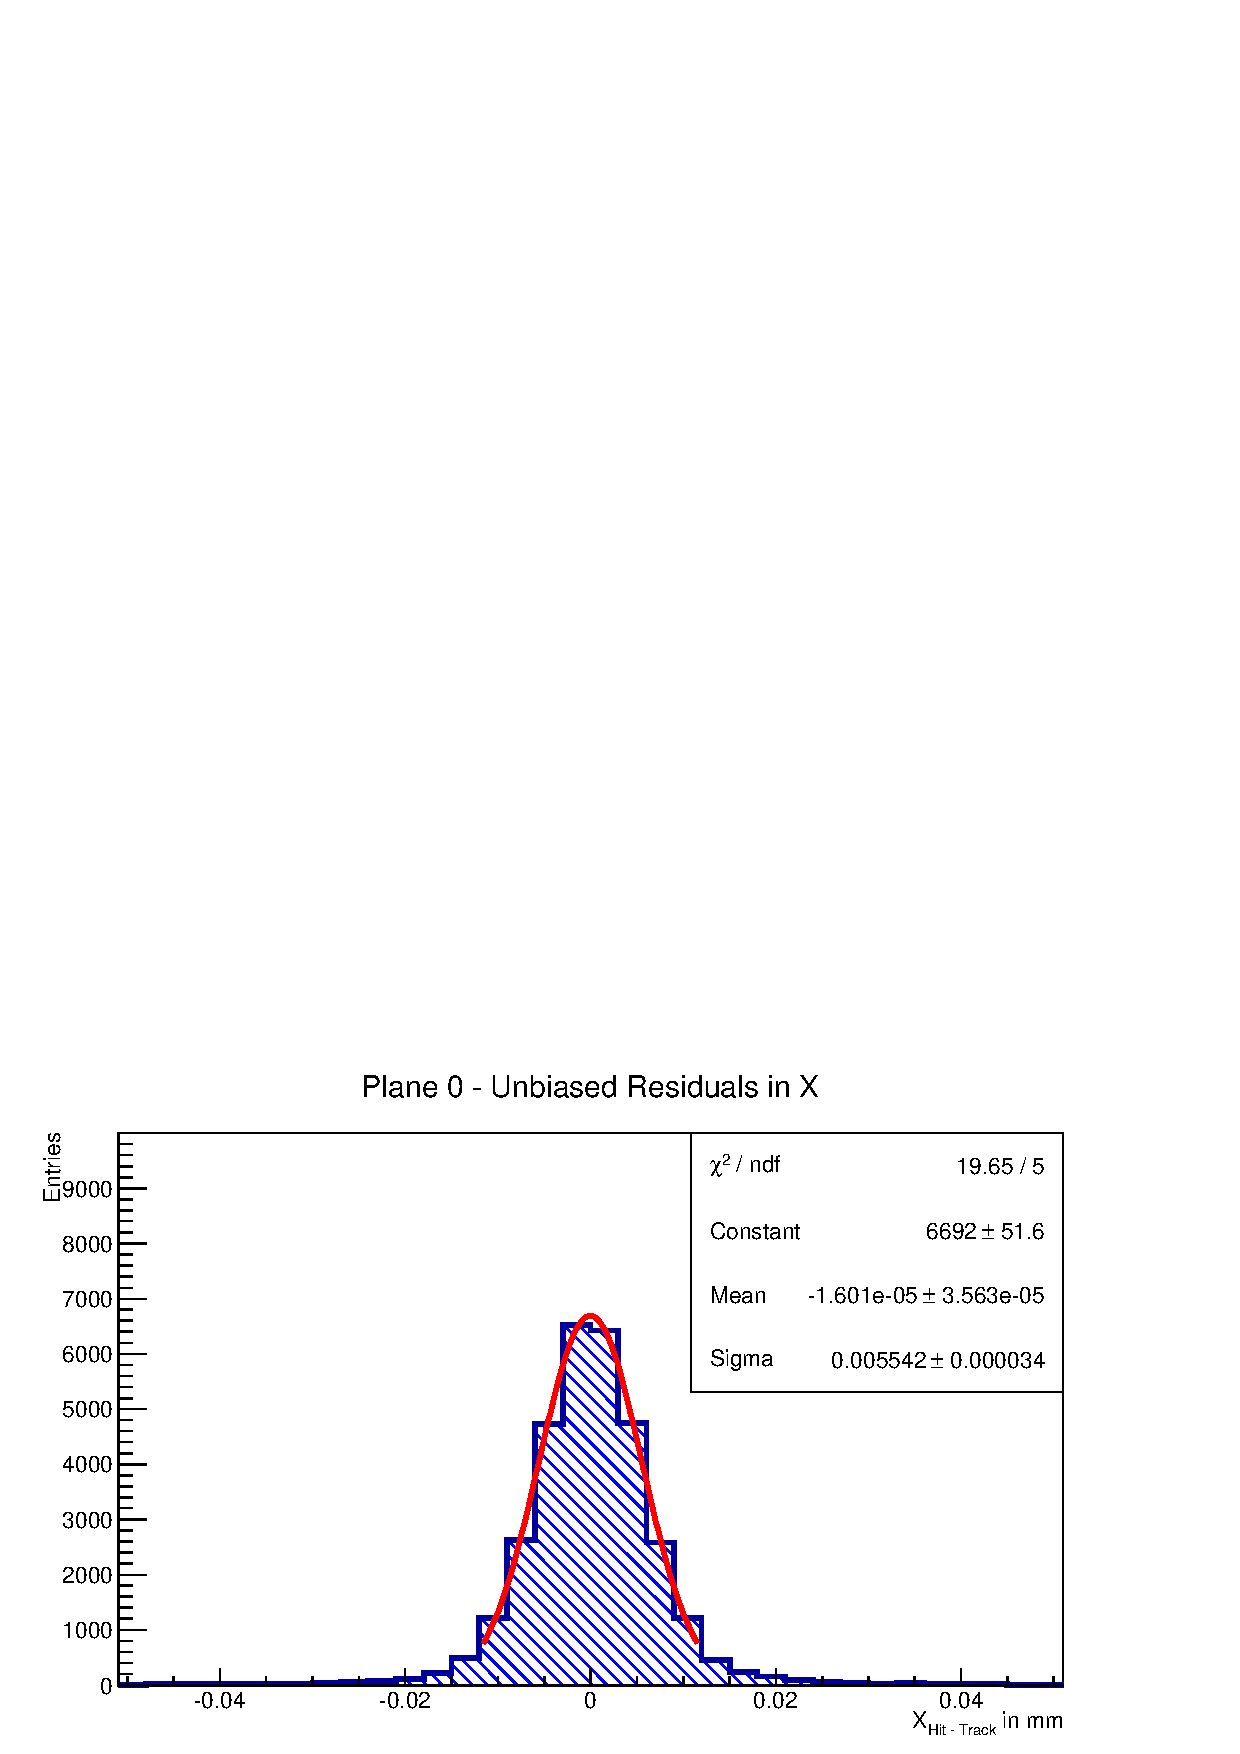
\includegraphics[width=0.45\textwidth]{figures/resis_upstream/0x.pdf}
  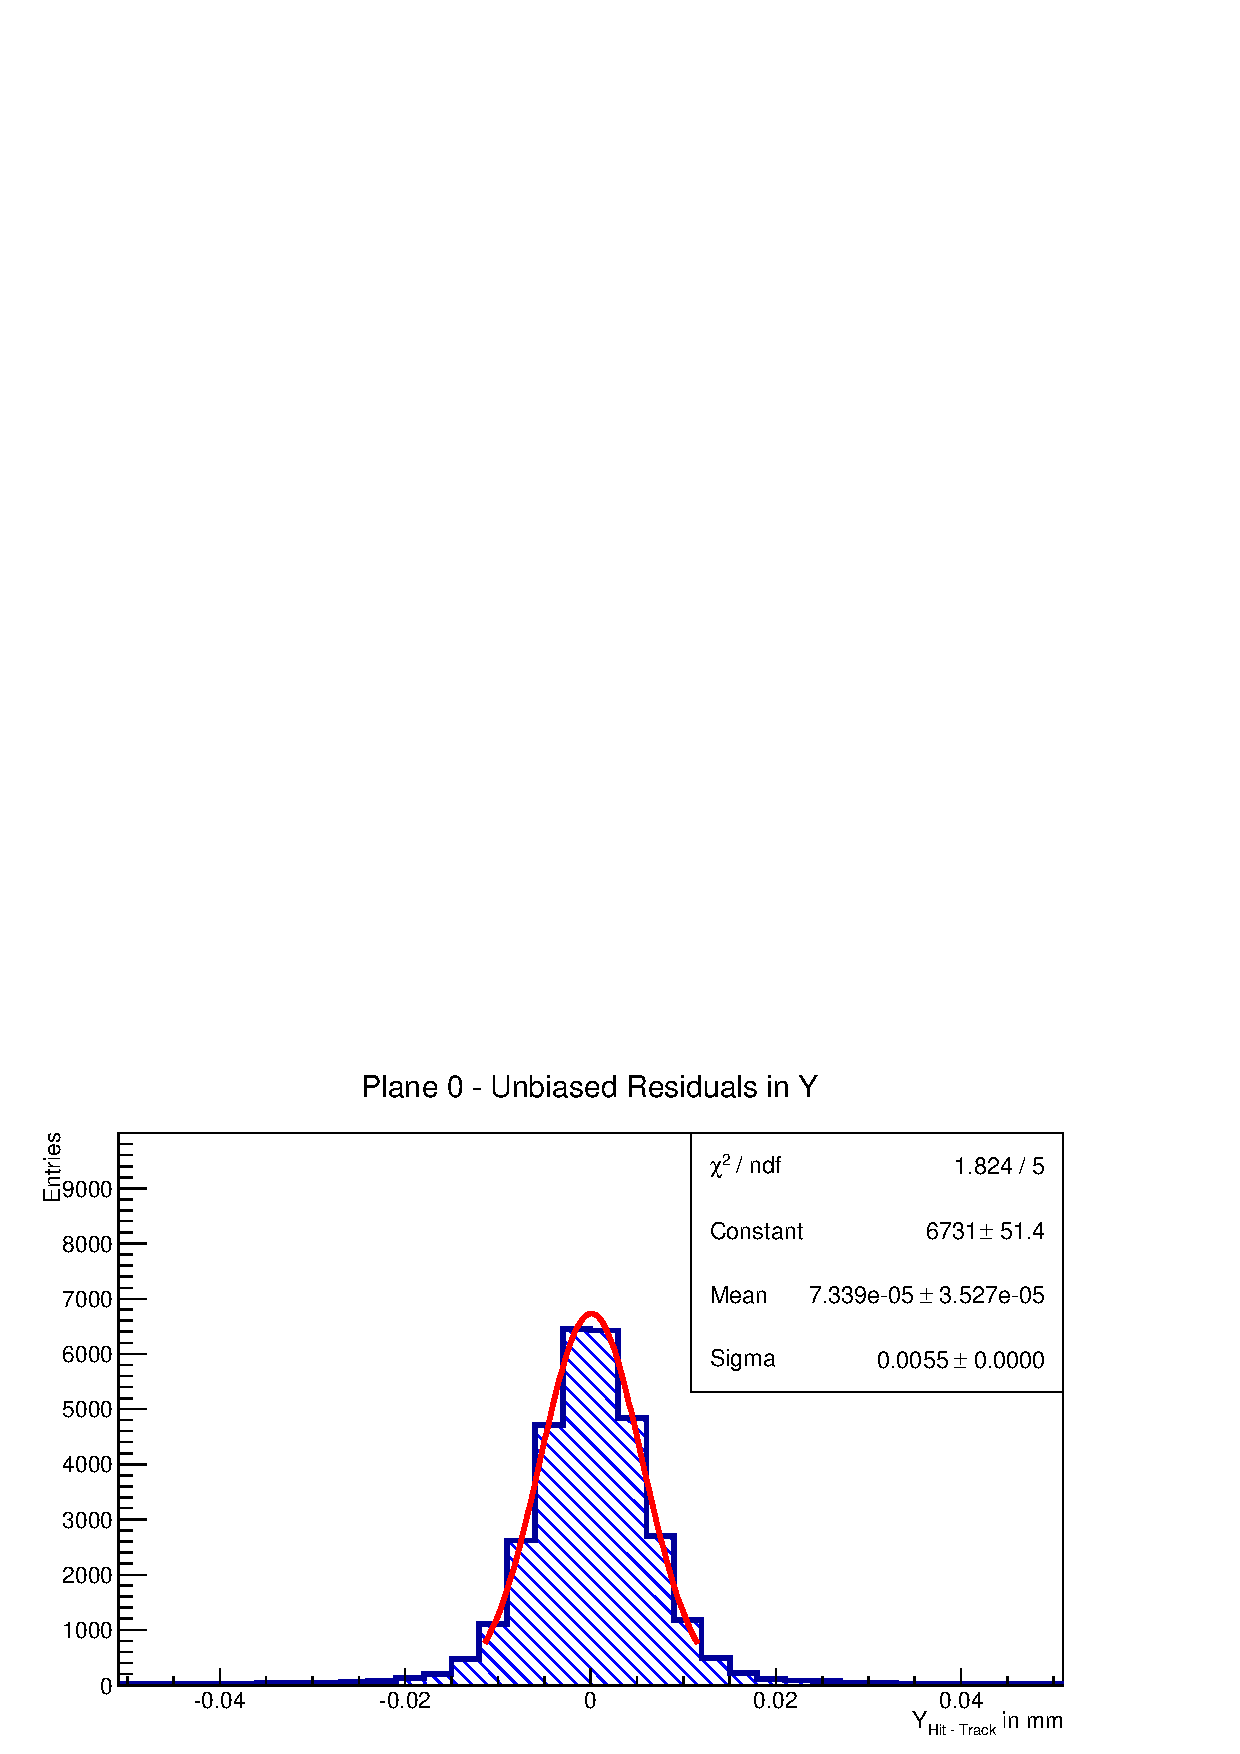
\includegraphics[width=0.45\textwidth]{figures/resis_upstream/0y.pdf}
  %\includegraphics[width=0.45\textwidth]{figures/resis_upstream/1x.pdf}
  %\includegraphics[width=0.45\textwidth]{figures/resis_upstream/1y.pdf}
  %\includegraphics[width=0.45\textwidth]{figures/resis_upstream/2x.pdf}
  %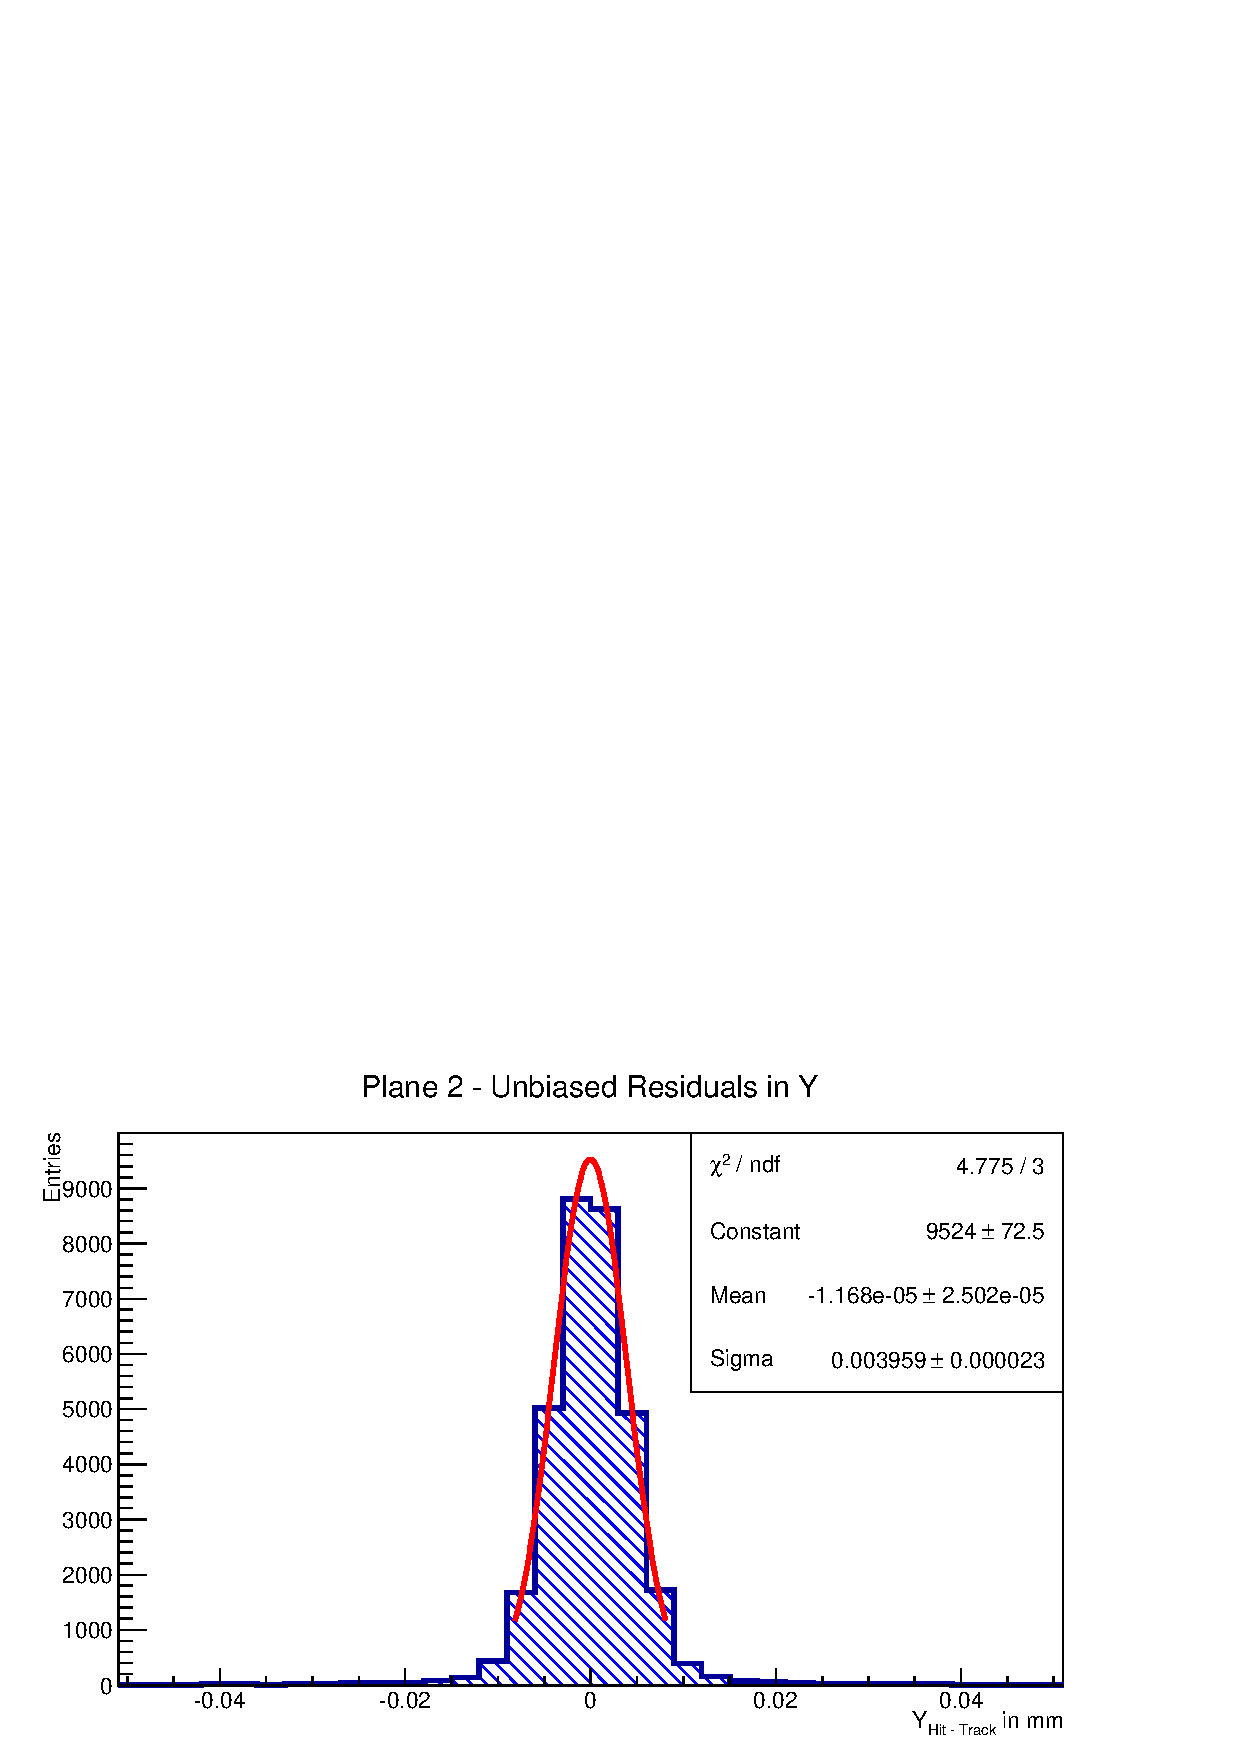
\includegraphics[width=0.45\textwidth]{figures/resis_upstream/2y.pdf}
  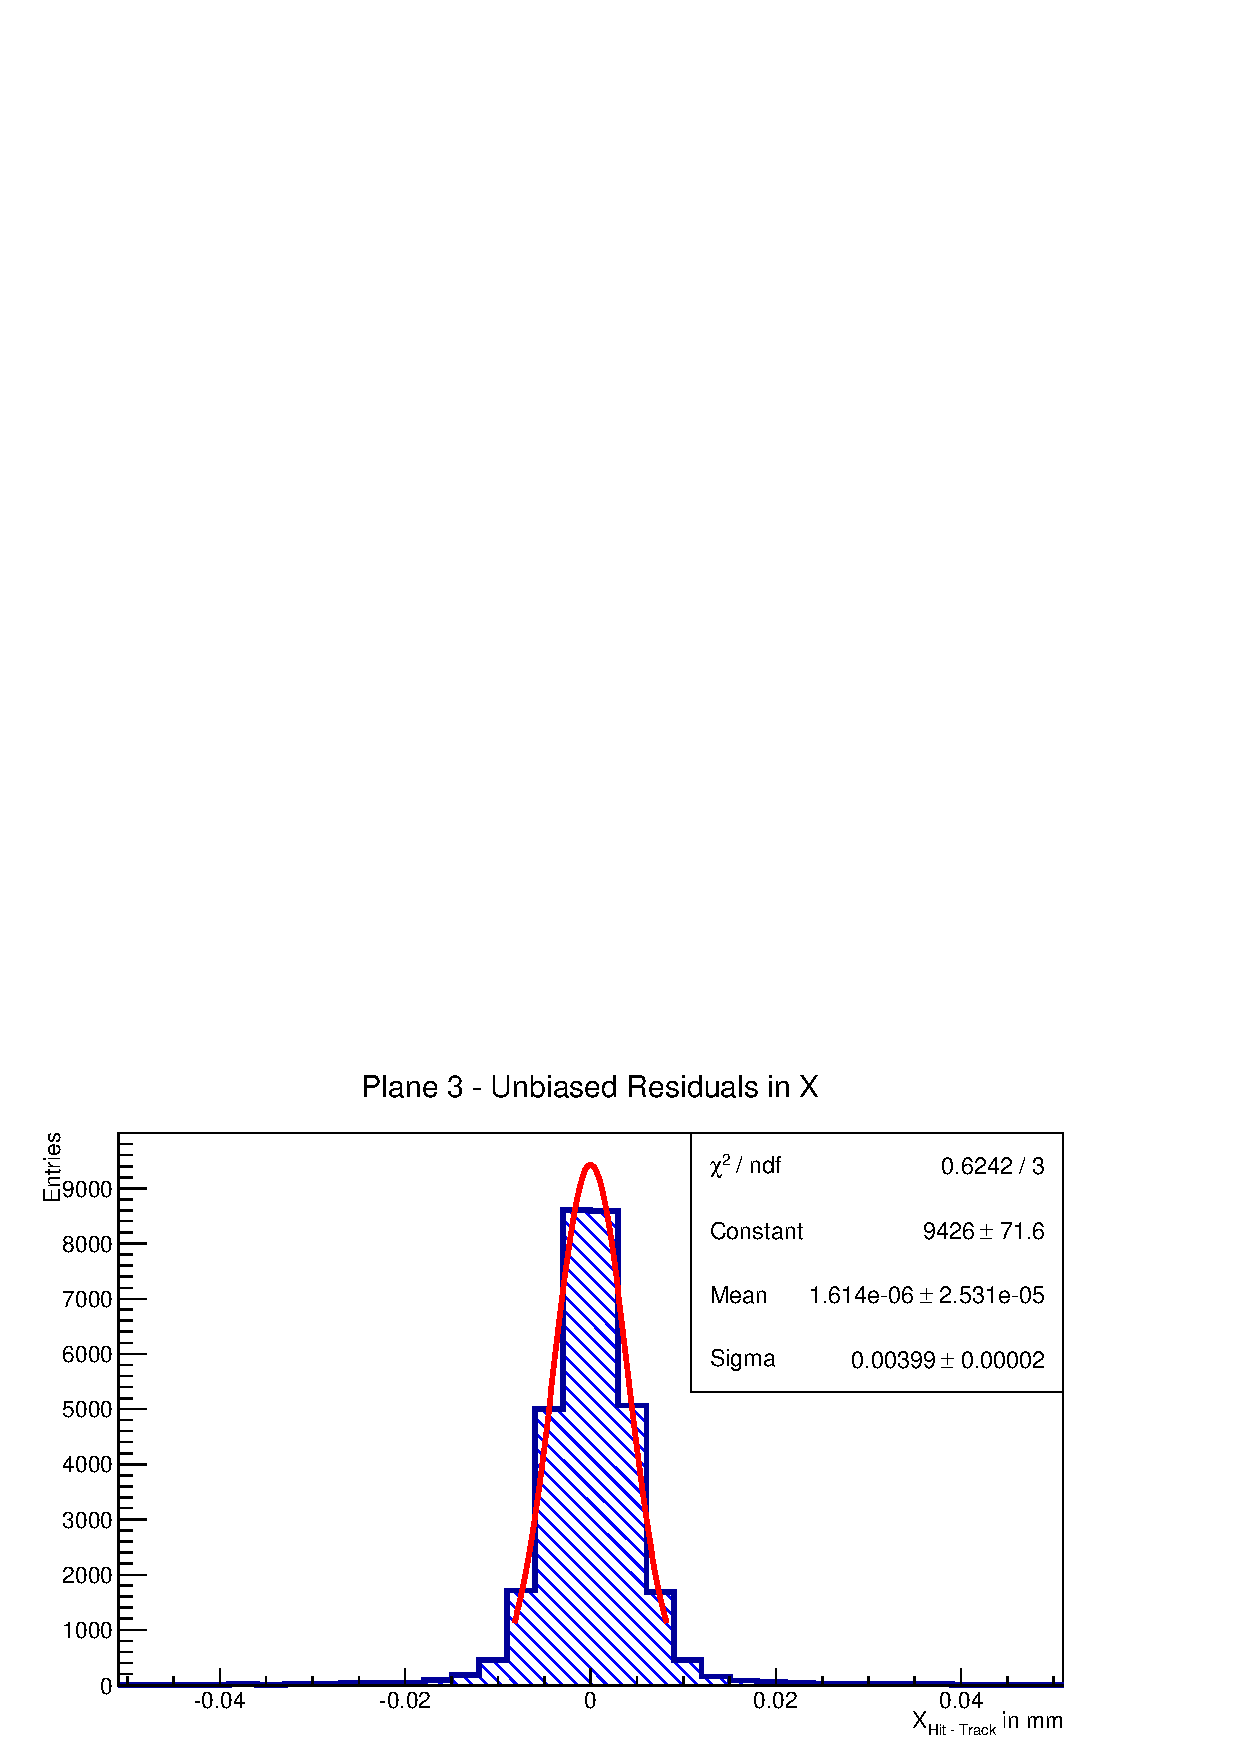
\includegraphics[width=0.45\textwidth]{figures/resis_downstream/3x.pdf}
  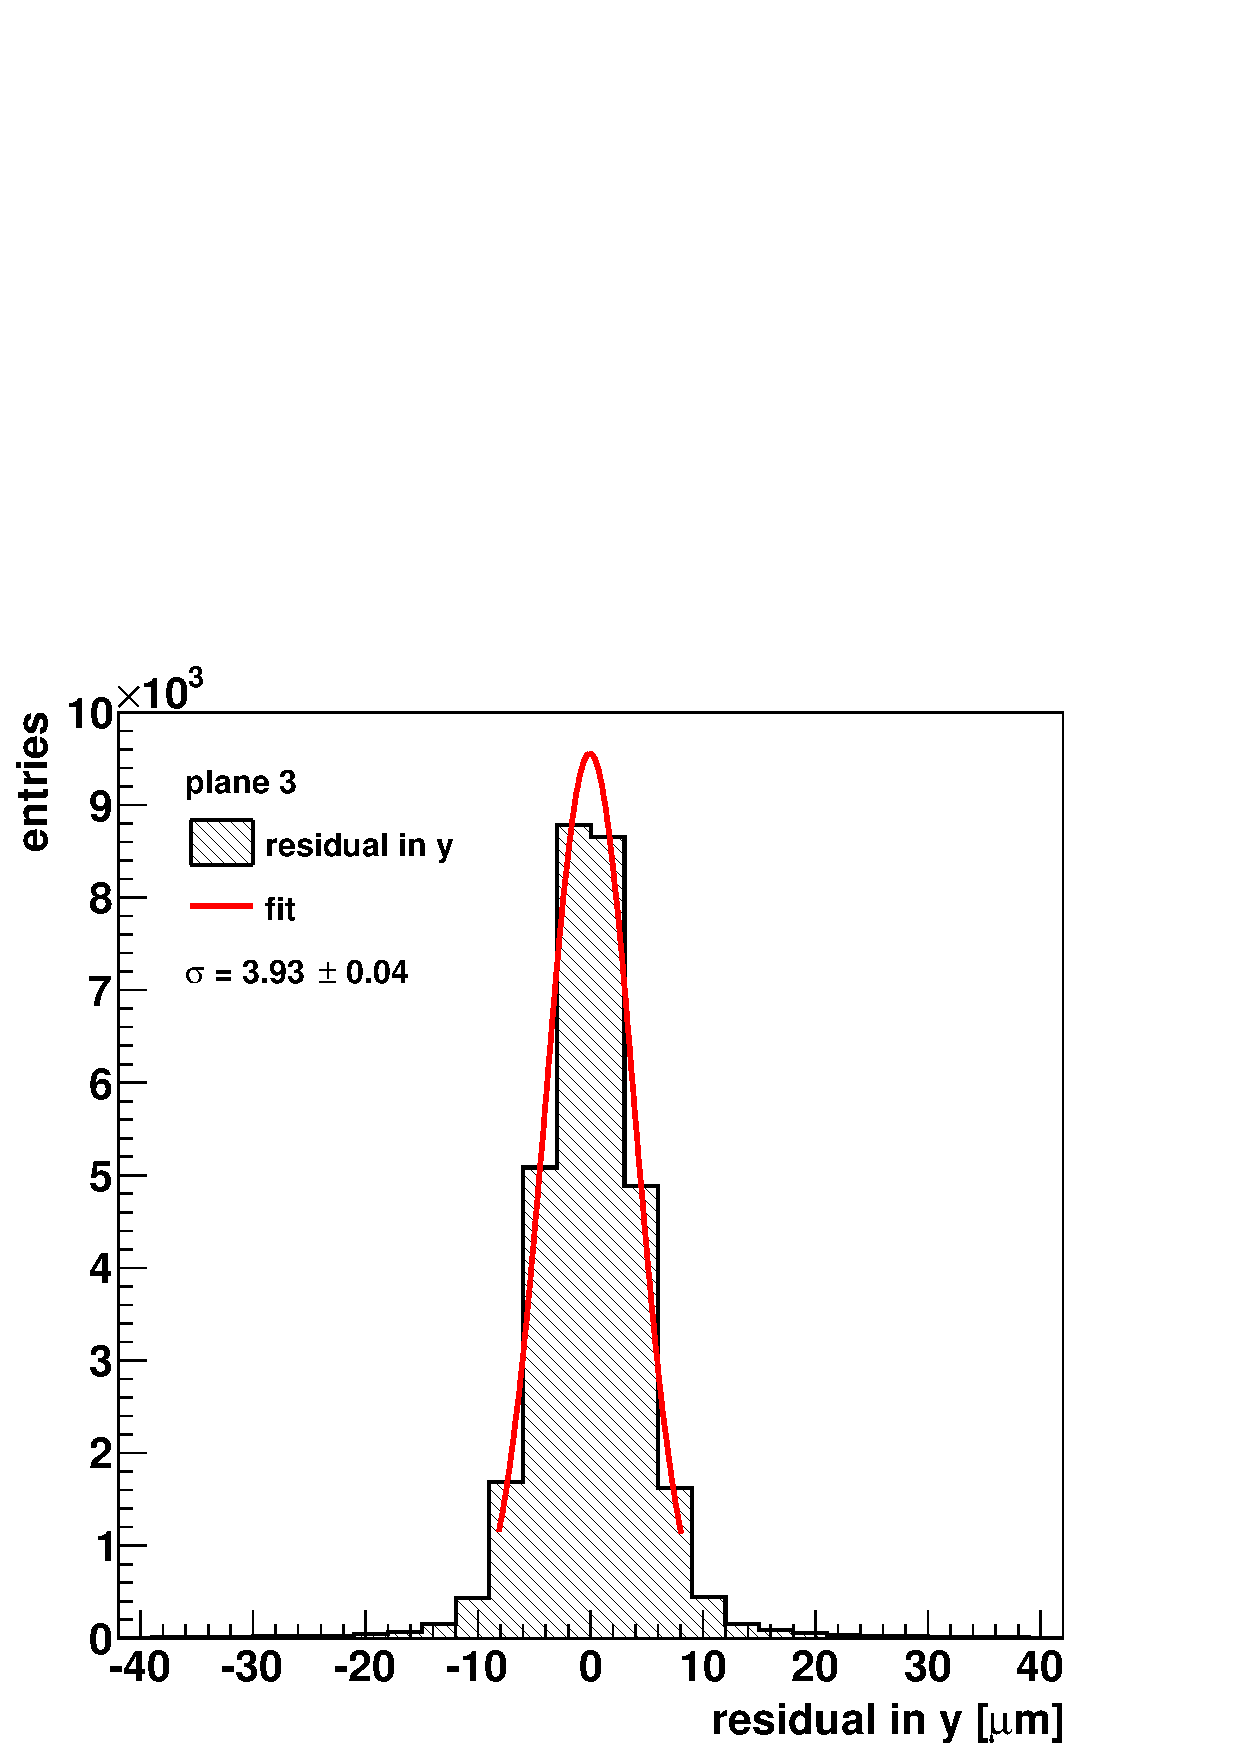
\includegraphics[width=0.45\textwidth]{figures/resis_downstream/3y.pdf}
  %\includegraphics[width=0.45\textwidth]{figures/resis_downstream/4x.pdf}
  %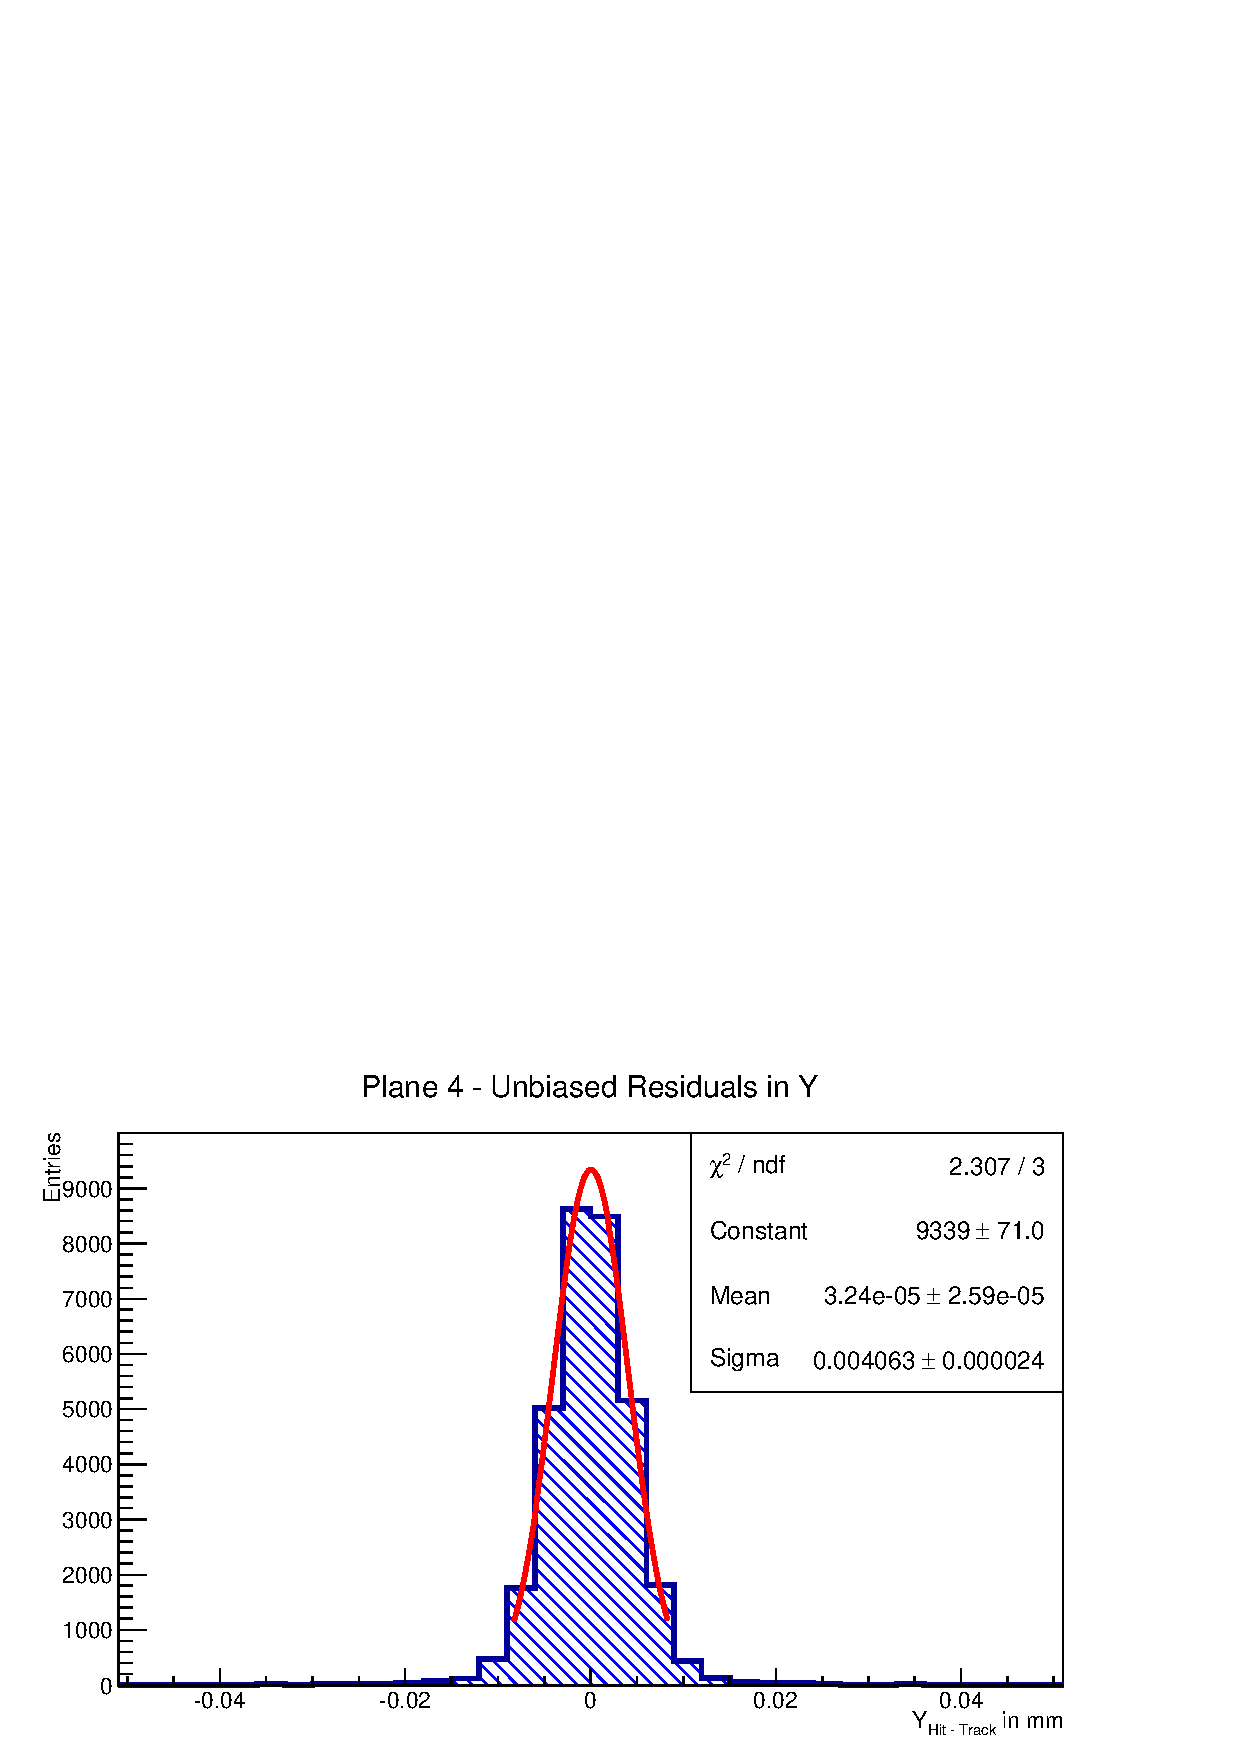
\includegraphics[width=0.45\textwidth]{figures/resis_downstream/4y.pdf}
  %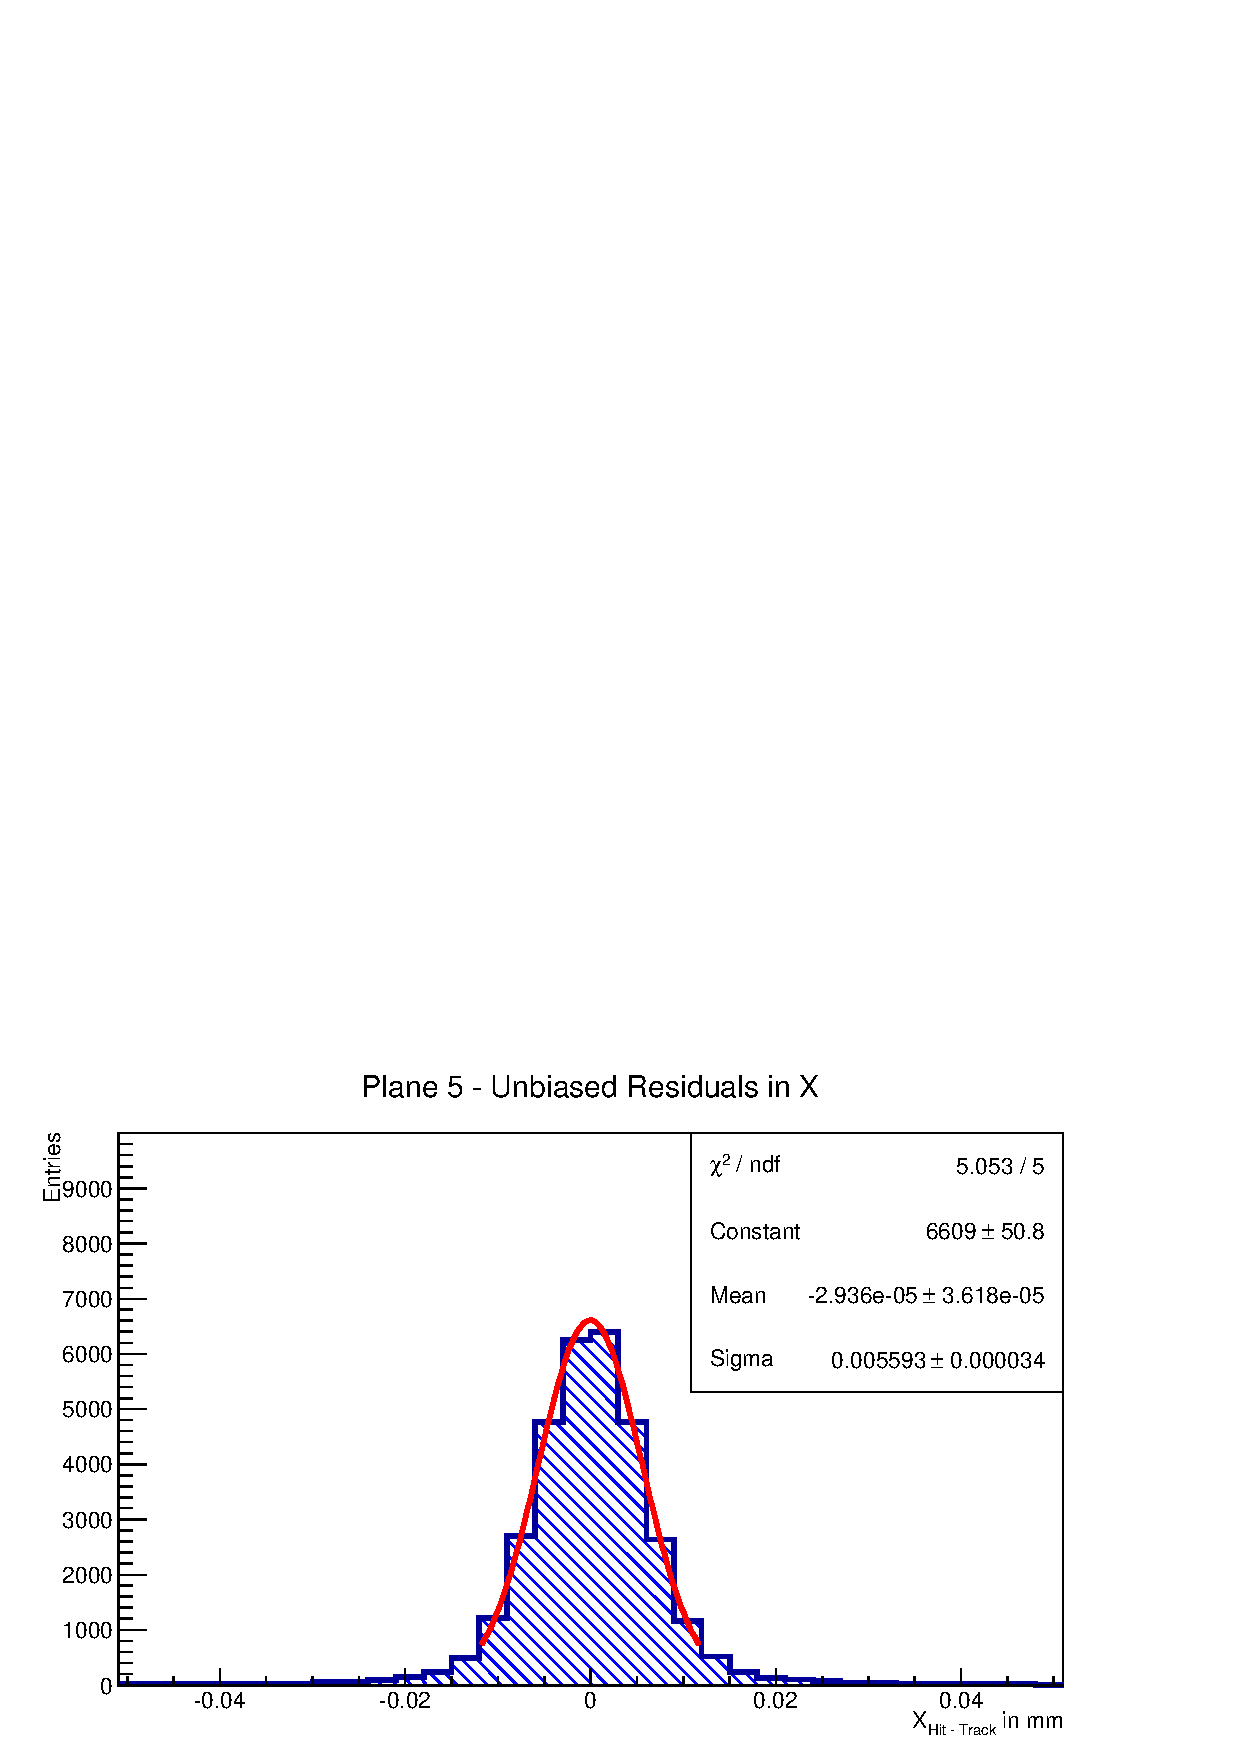
\includegraphics[width=0.45\textwidth]{figures/resis_downstream/5x.pdf}
  %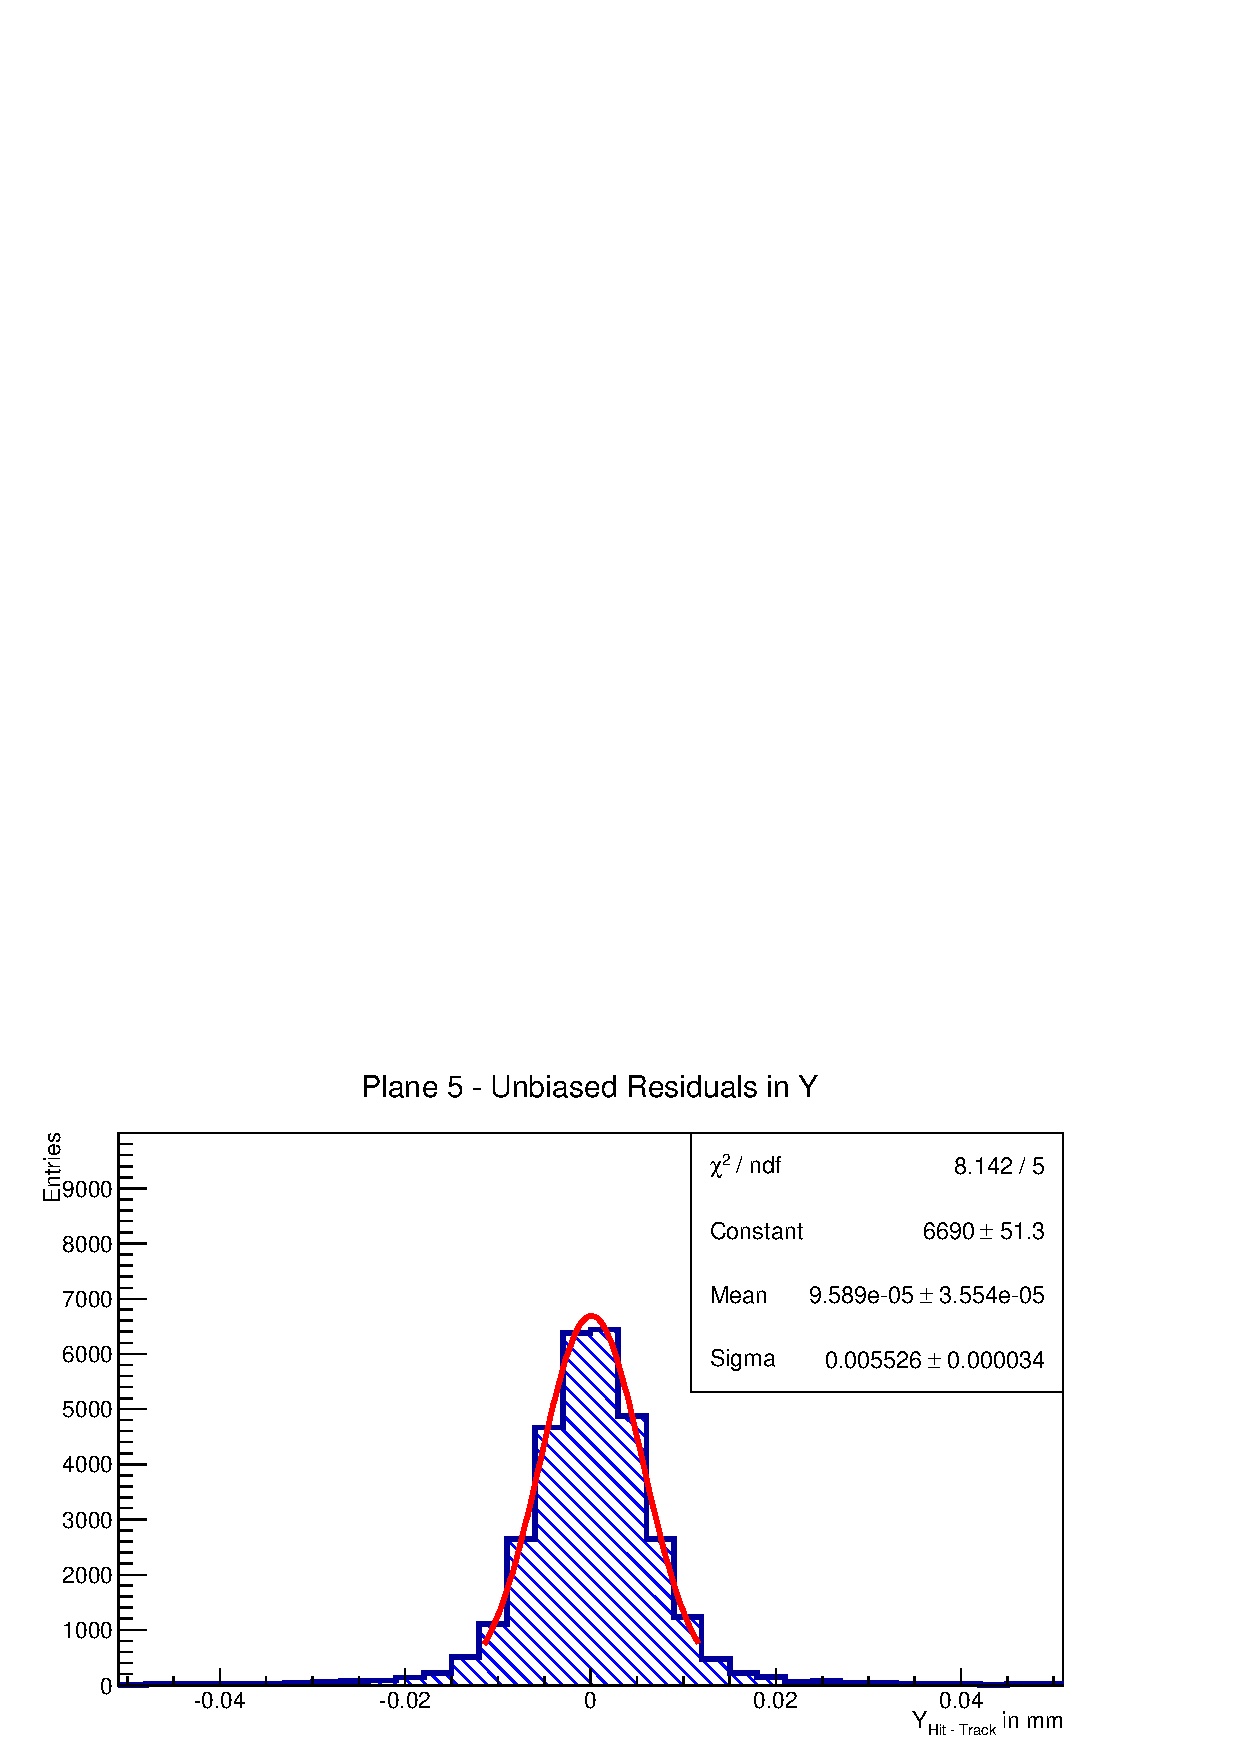
\includegraphics[width=0.45\textwidth]{figures/resis_downstream/5y.pdf}
  \caption[Residual examples to determine the $\Datura$ telescope's resolution~\cite{ref:thomas}]{Residual examples to determine the $\Datura$ telescope's resolution from the upstream lever arm.
From top to bottom: The measured residuals for planes $0$ and $3$, left for $x$ direction, right for $y$ direction.
Each sensor plane was considered as a passive layer during the track reconstruction. Images from~\cite{ref:thomas}.}
  \label{fig:residualexample1}
\end{figure}

Figure~\ref{fig:residualexample1} shows an example of residual distributions for a telescope sensor spacing of $20\,\milli\meter$,
 a beam momentum of $5\,\giga\electronvolt$ and a sensor threshold setting of $6$.
The residual distributions for the outer planes $0$ and $5$ are wider than the distributions obtained from the inner sensors.
This is due to the fact that the track extrapolation to the inner sensors is done from both sides, hence will be comparatively more precise than for the outer sensors,
 where the extrapolation can only be performed from one direction. 
In all cases, the distributions are fitted with a Gaussian, from which the residual width $\sigma_{\textrm{meas}}$ is determined.
It is noted, that the residuals feature non-Gaussian tails, as is expected from the underlying physics of the scattering mechanism. 
The measured resolution is defined here as the width of a Gaussian fit on middle 90\,\% of the residuals. 



% \begin{figure}[hbtp]
% \centering
% 
% \caption[Residual examples to determine the DATURA telescope's
% resolution. Downstream lever arm]{Residual examples to determine the DATURA
% telescope's resolution from the downstream lever arm. From top to bottom: The
% measured residuals for planes $3$, $4$ and $5$, left for $X$ direction, right
% for $Y$ direction. Each sensor plane was considered as a passive layer during
% the track reconstruction.}
% \label{fig:residualexample2}
% \end{figure}

By using a $\chi^{2}$ minimization method, the intrinsic resolution of the $\Mimosa$ telescope sensors was calculated, with the contribution $\Delta \chi^2_{i,j}$ from plane $i$ in dimension $j$ defined as

\begin{equation}
\Delta \chi^2_{i,j} = \left( \frac{y_{i,j} - p_{i,j}}{\sigmai} \right)^2 +
\left( \frac{\theta_{\textrm{i,j}} - \theta_{i-1,j}}{\Theta_{0}} \right)^2 \,.
\end{equation}

\noindent The measured hit position is denoted by $y_{i,j}$, the position extrapolated from the track by $p_{i,j}$. $\theta_{i-1,j}$ and $\theta_{i,j}$ are the angles between the nominal beam direction
 and the track direction. The former is the track angle entering plane $i$, the latter the angle of the outbound track segment.
$\sigma_{i,j}$ and $\Delta \theta_{i,j}$ are the intrinsic resolution of sensor plane $i$ in dimension $j$ and the width of the multiple scattering distribution,
 according to equation~(\ref{eq:multiplescattering}), respectively.
\\comments hj: \\
- chi2 minimisation needs better explanations. 
% - Is this done after track fitting? so tracks are not altered during this process? -> No \\
%- Are you really using $\sigma_{i,j}$? Or just one $\sigma_{\textrm{intrinsic}}$? -> Just sigma intrinsic\\
%- same for $\Delta \Theta_{i,j}$. Shouldnt it be just one $\Theta_0$ from Eq.~(4) ? YES\\
%- difference in theta for straight tracks ?!
%- What about the actual summing? Is the chi2 summed over many tracks? And then over n planes leaving out the $i$-th? so something like:

Resulting from this minimisation, the intrinsic resolution $\sigma_{\textrm{M26}}$ of the $\Mimosa$ sensors is \allowbreak$\left( 3.42\,\pm\, \allowbreak 0.12 \right)\,\micro\meter$
 and $\left( 3.44\,\pm\,0.10 \right)\,\micro\meter$ for a plane spacing of $20\,\milli\meter$ and $150\,\milli\meter$, respectively.
The results for both a tighter plane spacing of $20\,\milli\meter$ and a wider spacing of $150\,\milli\meter$ are shown in figure~\ref{fig:smiley} for each plane separately. 
In both cases, an error of $2.5\,\milli\meter$ on the plane distance $\Delta_{\textrm{z}}$ was assumed.
For both geometries, the expected resolution of $\approx\,3.5\,\micro\meter$, according to reference~\cite{ref:mimosa26}, is confirmed.
The underlying assumptions in the method presented here are:

\begin{figure}[tbp]
  \centering
  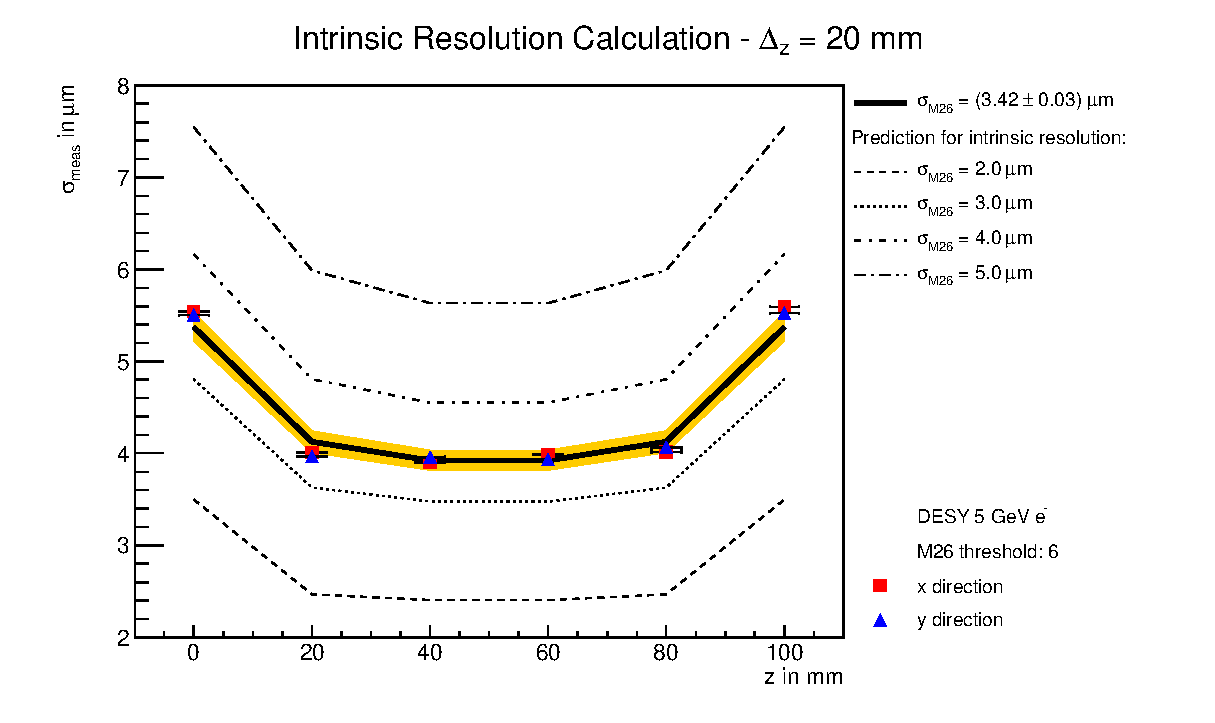
\includegraphics[width=0.49\textwidth]{figures/20} % was thin_smiley.pdf
  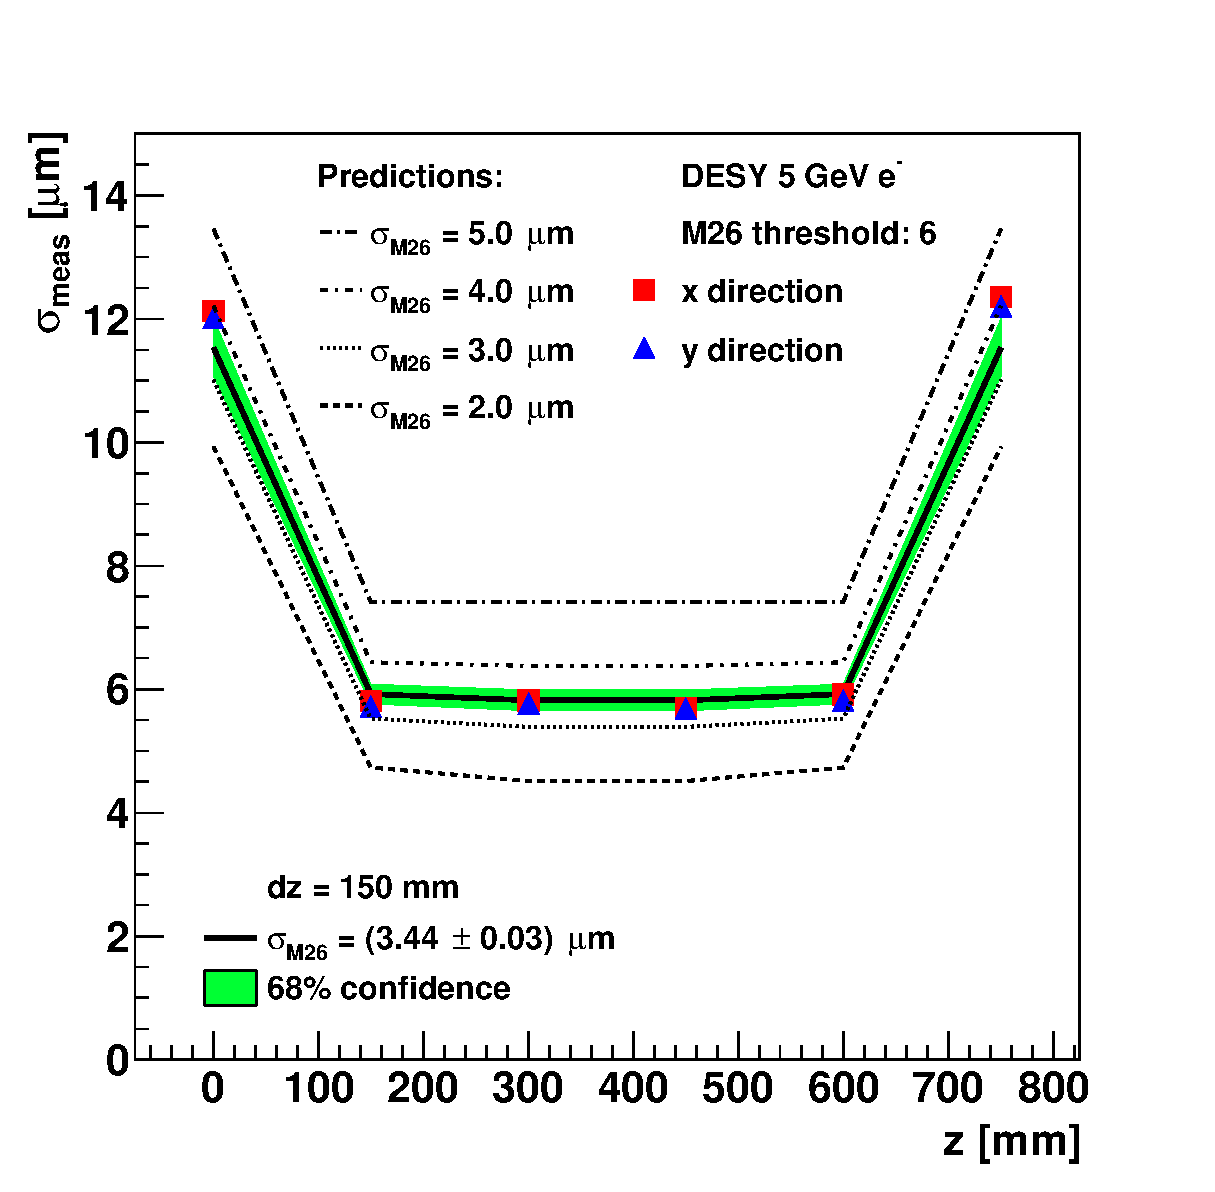
\includegraphics[width=0.49\textwidth]{figures/150} % was wide_smiley.pdf
  %\caption[Intrinsic telescope sensor resolution at $20\,\milli\meter$ and $150\,\milli\meter$ plane spacing~\cite{ref:thomas}]{Intrinsic telescope sensor resolution at $20\,\milli\meter$ (top)
  % and $150\,\milli\meter$ (bottom) plane spacing.
  \caption[The measured residual widths of each telescope plane.]{The measured residual widths of each telescope plane are shown in both the $x$ and $y$ direction for the $20\,\milli\meter$ (top)
   and $150\,\milli\meter$ (bottom) plane spacing.
  Dotted and dashed lines indicate the expected measured widths, if the intrinsic resolution is assumed to differ upward or downward from the real one. 
  The yellow band indicates the resulting intrinsic telescope sensor resolution including errors.
  For both telescope geometries, data was taken at a sensor threshold setting of $6$ and with $5\,\giga\electronvolt$ electrons.
  Images from~\cite{ref:thomas}.}
  \label{fig:smiley}
\end{figure}



\begin{itemize}
\item The intrinsic resolution $\sigmai$ of all sensor planes is assumed to be equal.
As the discriminator thresholds are set for subframes of each plane individually, however, this is not necessarily true.
Figure~\ref{fig:resivsenergy_thresh} shows the dependence of $\sigmai$ on the applied threshold.

\item The multiple scattering term in equation~(\ref{eq:telescoperesolutionequation_2}) is only calculated considering the nominal sensor thicknesses, the air between sensor planes,
 and a $25\,\micro\meter$ thick capton foil on either side of each sensor.
The particle momentum assumed is the nominal beam momentum.

\item Residuals are calculated using straight-line tracks only.
Inclined tracks, or a deflection of tracks in planes or scattering material, are not considered.
\end{itemize}

Figure~\ref{fig:resivsenergy_thresh} (A) shows the calculated intrinsic telescope sensor resolution for different beam energies, plane distances and applied sensor thresholds.
The minimum of the $\Mimosa$ sensors' intrinsic resolution is reached for a threshold setting of $6$.
While the measured residual width for wider sensor spacings or lower beam momenta is higher, as can be seen in figure~\ref{fig:smiley},
 these effects are accounted for in equation~(\ref{eq:telescoperesolutionequation}) by the terms $\sigma_{\textrm{Tel}}^2$ and $\sigma_{\textrm{MS}}^2$.
Because of this, the difference in intrinsic sensor resolution between configurations at any given threshold is only approximately $\pm\,0.15\,\micro\meter$, which is well within the errors.
From equation~(\ref{eq:telescopepointing}) the optimal track pointing resolution $\sigma_{\textrm{Tel}}$ of the $\Datura$ telescope without multiple scattering
 can therefore be given as $\left( 1.40 \pm 0.05 \right)\,\micro\meter$.
Measurements by Behr\,\cite{ref:j.behrmeasurements}, taken at high thresholds $>\,10$ show comparable results of $\sigma_{\textrm{M26}} = (4.35\,\pm\,0.10)\,\micro\meter$.

\begin{figure}[tbp]
  \centering
  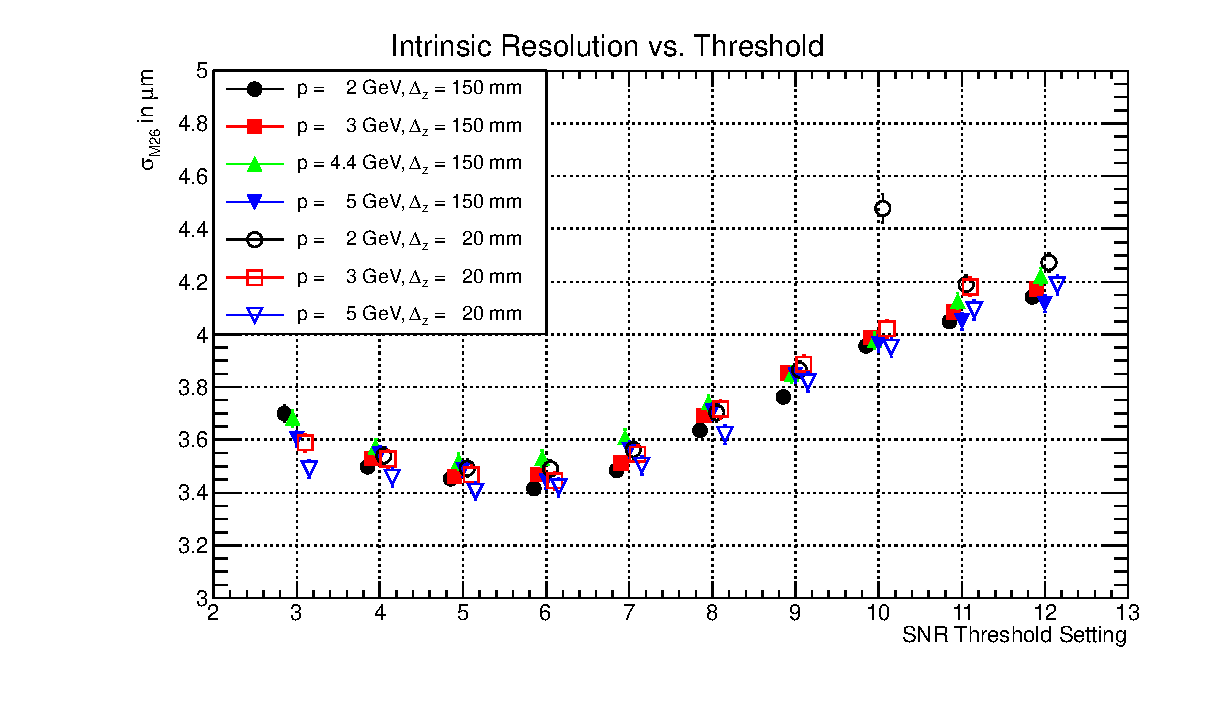
\includegraphics[width=0.49\textwidth]{figures/resi_vs_thresh}	\put(-175,100){(A)} % was resi_thresh_errors
  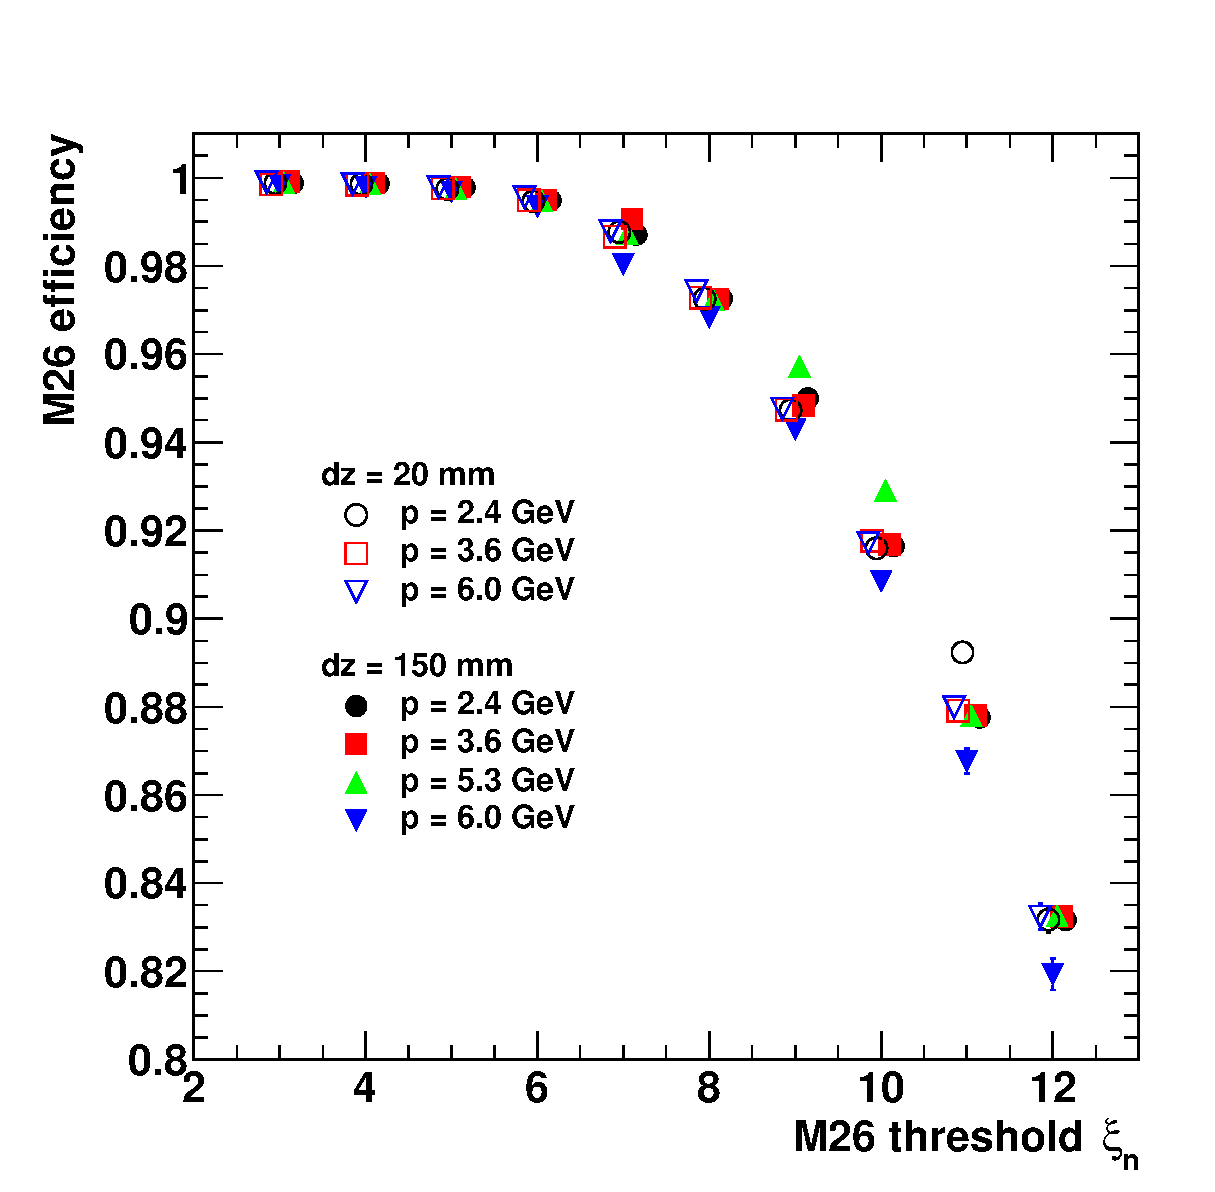
\includegraphics[width=0.49\textwidth]{figures/effi_thresh}		\put(-175,100){(B)}
  \caption[Telescope intrinsic sensor resolution for different threshold settings, beam momenta and geometries~\cite{ref:thomas}]{
(A) The measured intrinsic resolution of the $\Datura$ telescope's $\Mimosa$ sensors $\sigma_{\textrm{M26}}$ for different beam momenta $p$, sensor spacing $\Delta_{\textrm{z}}$ and applied sensor threshold.
Some values are shifted on the x-axis for improved legibility.
(B) Average efficiency of all telescope sensors in both dimensions for different beam momenta and sensor spacing vs. applied threshold.
An efficiency decline with increasing threshold can be observed.
Some values are shifted on the $x$ axis for improved legibility. 
Images from~\cite{ref:thomas}.}
  \label{fig:resivsenergy_thresh}
\end{figure}

The signal-to-noise threshold applied to each telescope sensor is a critical parameter for a telescope's performance.
A higher threshold cuts into the signal, thus reducing the amount of clusters found on each plane and therefore reducing the amount of re-constructable tracks.
This reduces a sensor's efficiency.
A lower threshold allows for an increasing amount of noise hits to be wrongly identified as clusters.
This also leads to a broadening of the residual distributions and hence a worse resolution. 
%Figure~\ref{fig:effi} shows the efficiency distribution over a sensor plane.
The efficiency is defined as the ratio of tracks that have at least one hit above threshold in the vicinity of a reconstructed track on the DUT to the overall number of tracks.
As maximum distance $100\,\micro\meter$ is considered.
%A noisy pixel column at $Y \approx -8\,\milli\meter$ can be observed.
%This column was masked during the converter step in the \texttt{datura-noDUT} example and subsequently is not used during the analysis. 
%\\{comment hj: datura-noDUT is jargon}\\
%Disregarding this area, an overall average efficiency over $98\,\%$ is observed.
In figure~\ref{fig:resivsenergy_thresh} (B), the efficiency dependence on the sensor threshold is shown, for various beam momenta and sensor spacings.
Efficiencies are averaged for all six sensor planes and both spatial coordinates, resulting in negligible statistical errors. 
In all cases, the efficiency is $\ge\,98\,\%$ up to a threshold setting of 7.
With increasing threshold, the efficiency declines, until an efficiency of $86\,\%$ for threshold $12$ is reached.
The difference between momenta and plane spacings is due to multiple scattering and increased telescope resolution.

%\begin{figure}[tbp]
%  \centering
%  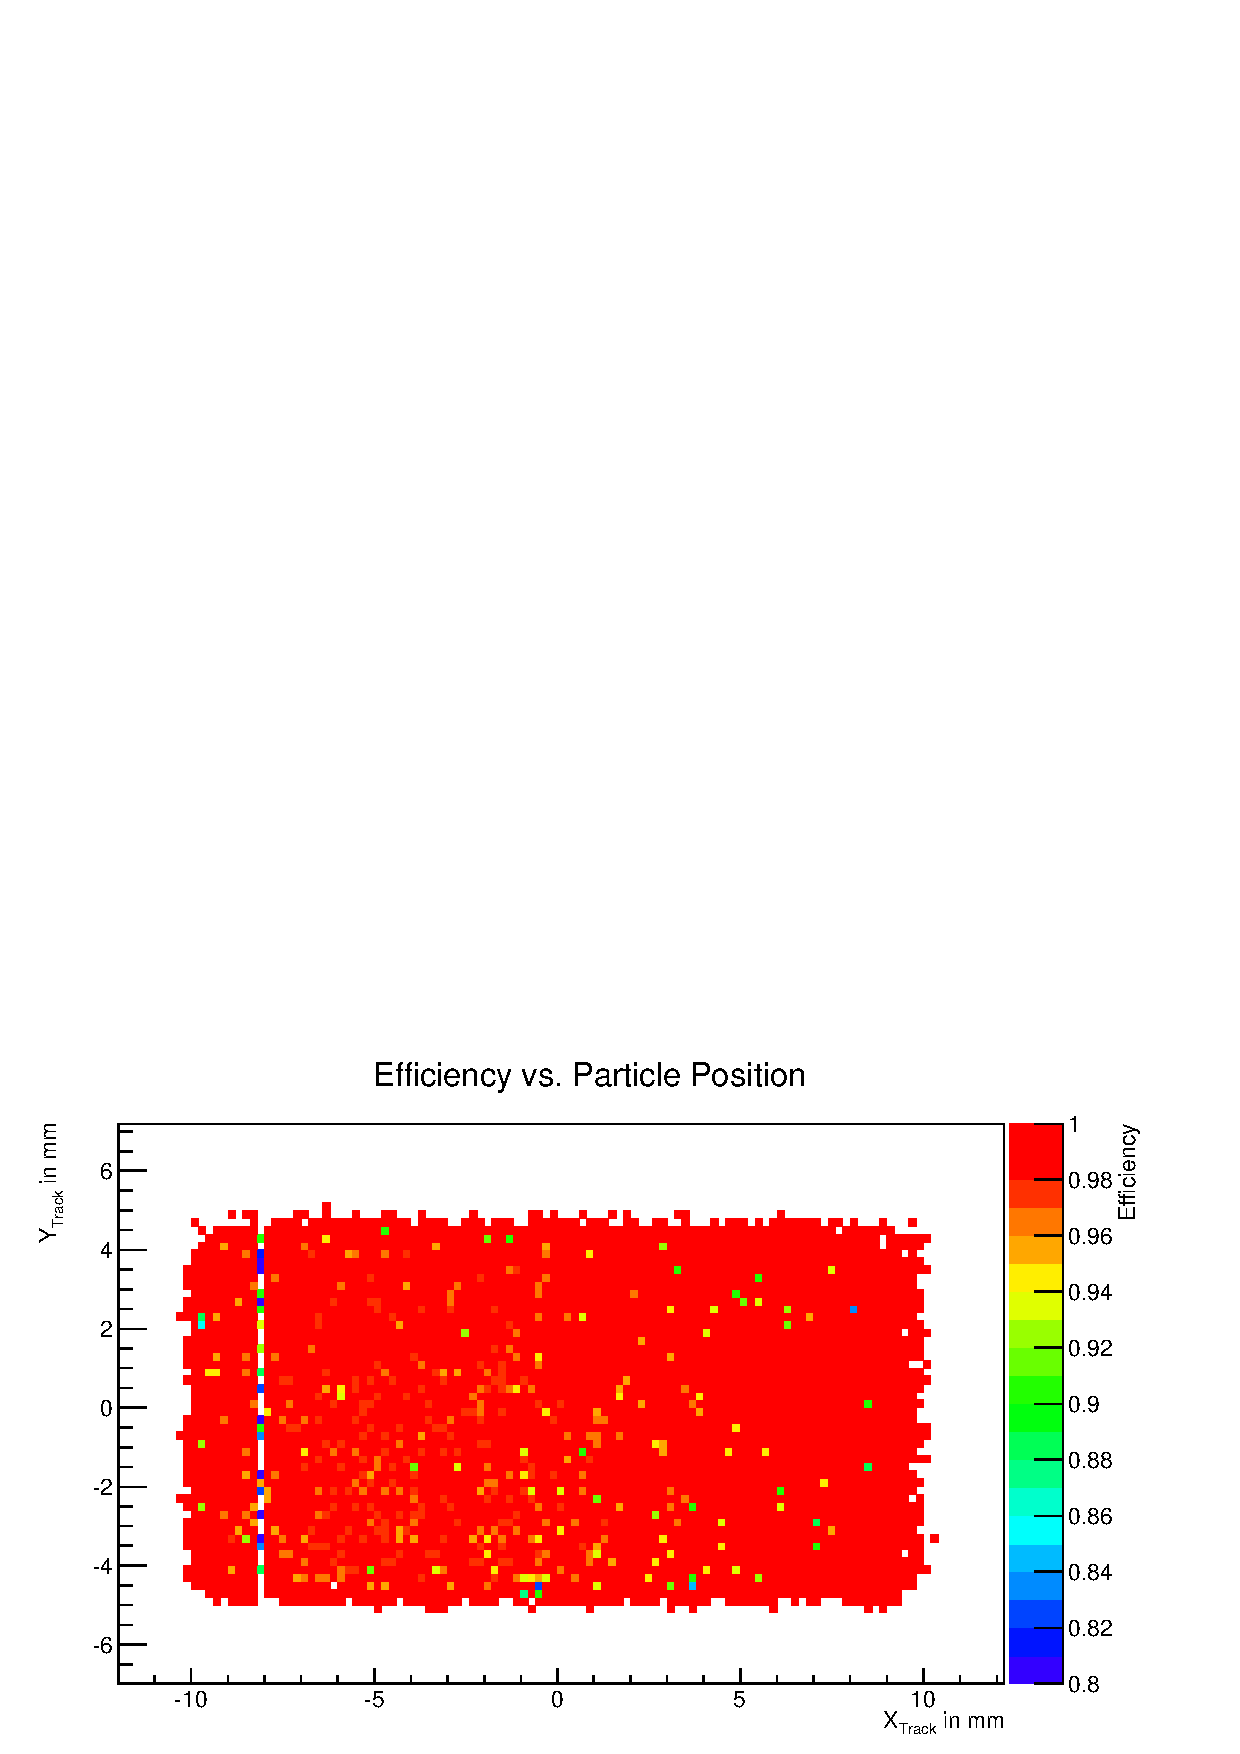
\includegraphics[width=\textwidth]{figures/plane3_effi_run37.pdf}
%  \caption[Telescope sensor efficiency~\cite{ref:thomas}]{Efficiency of telescope sensor plane $3$ at a threshold of $7$ and $5\,\giga\electronvolt$ beam momentum.
%Image from~\cite{ref:thomas}.}
%\label{fig:effi}
%\end{figure}



%\begin{figure}[tbp]
%  \centering
%  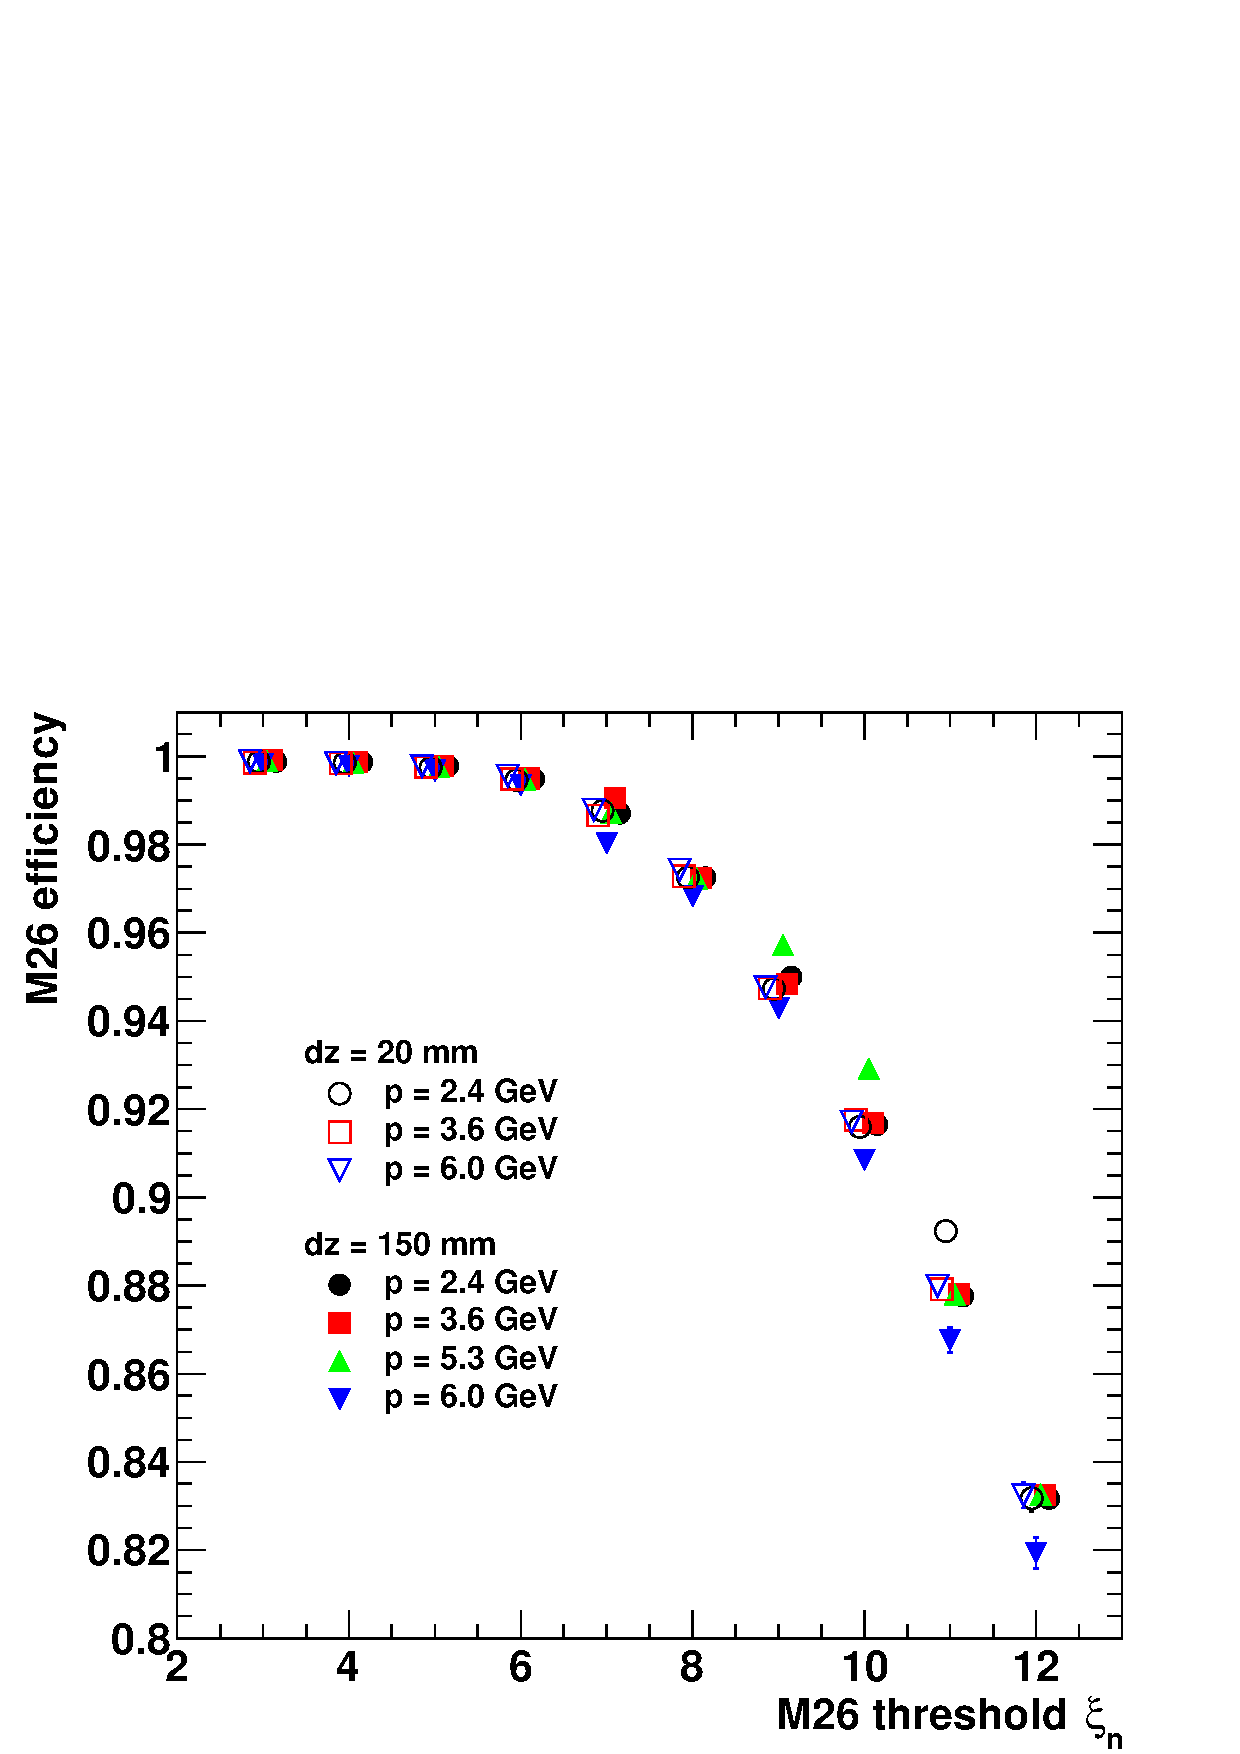
\includegraphics[width=\textwidth]{figures/effi_thresh.pdf}
%  \caption[Overall telescope sensor efficiency vs. threshold for different beam momenta and sensor spacings~\cite{ref:thomas}]{
%Average efficiency of all telescope sensors in both dimensions for different beam momenta and sensor spacing vs. applied threshold.
%An efficiency decline with increasing threshold can be observed.
%Some values are shifted on the $x$ axis for improved legibility.
%Image from~\cite{ref:thomas}.}
%\label{fig:effi_thresh}
%\end{figure}



\subsection{Resolution predictions using General Broken Lines}

With the measured intrinsic resolution at hand, and the knowledge about the amount of material of the sensor planes, predictions of the expected pointing resolution at the actual DUT position can be made. 
Therefore, it is possible to calculate a priori the optimal telescope geometry for a certain measurement set-up. 
Pointing resolutions in this section therefore therefore refer to the achievable pointing resolution using a ``symmetric six planes plus DUT'' configuration,
 cf.~figure~\ref{fig:datura_sketch}, if not stated otherwise.
Using the GBL formalism \cite{Kleinwort-2012,Blobel-2006}, the pointing resolution is analytically calculated at desired points of interest along the particle trajectory. 
Assuming $\epsmimo = 0.00071$, the pointing resolution at the DUT for four different DUT material budgets $\epsdut$ is plotted as a function of the spacing $\dzdut$
 for two fixed values of $\dz = 20\,\milli\meter$ and $50\,\milli\meter$ in figure~\ref{fig:CalcResos_dzdut}. 
Plots are provided for DESY\,II beam energies (left) and SPS energies (right). 
All plotted resolution functions are monotonically increasing with increasing $\dzdut$. 
Therefore, the optimal position of the $\Mimosa$ planes nearest to the DUT need to always be installed as close to the DUT as possible in order to achieve the best possible resolution. 
Also from figure~\ref{fig:CalcResos_dzdut} it can be seen, that the optimal plane spacing $\dz$ depends on the actual material budget of the DUT and the actual space needed for the DUT, hence $\dzdut$.
E.g.~for a DUT with a material budget of $\epsdut = 0.001$ (black and red solid line) at 5\,GeV/$\cspeed$, a narrow configuration is preferred for $\dzdut < 70\,\milli\meter$,
 but a wide configuration for $\dzdut > 70\,\milli\meter$.
The position of the intersection depends on the material budget of the DUT and decreases with increasing material budget. 
In a wide configuration, the pointing resolution is limited to about $2.3\,\upmu\meter$, whereas in a narrow configuration a pointing resolution around $2.0\,\upmu\meter$ is achievable for thin DUTs.
At SPS energies, the resolution functions for the wide and the narrow configuration do not cross, with the narrow configuration being slightly better than the wide one.
However, the difference e.g.~for $\epsdut = 0.01$ is less than $300\,\nano\meter$ for $\dzdut = 100\,\milli\meter$.

\begin{figure}[tbp]
  \centering
  \includegraphics[width=0.49\textwidth]{figures/CalcResoVsDzdut_Desy_2}
  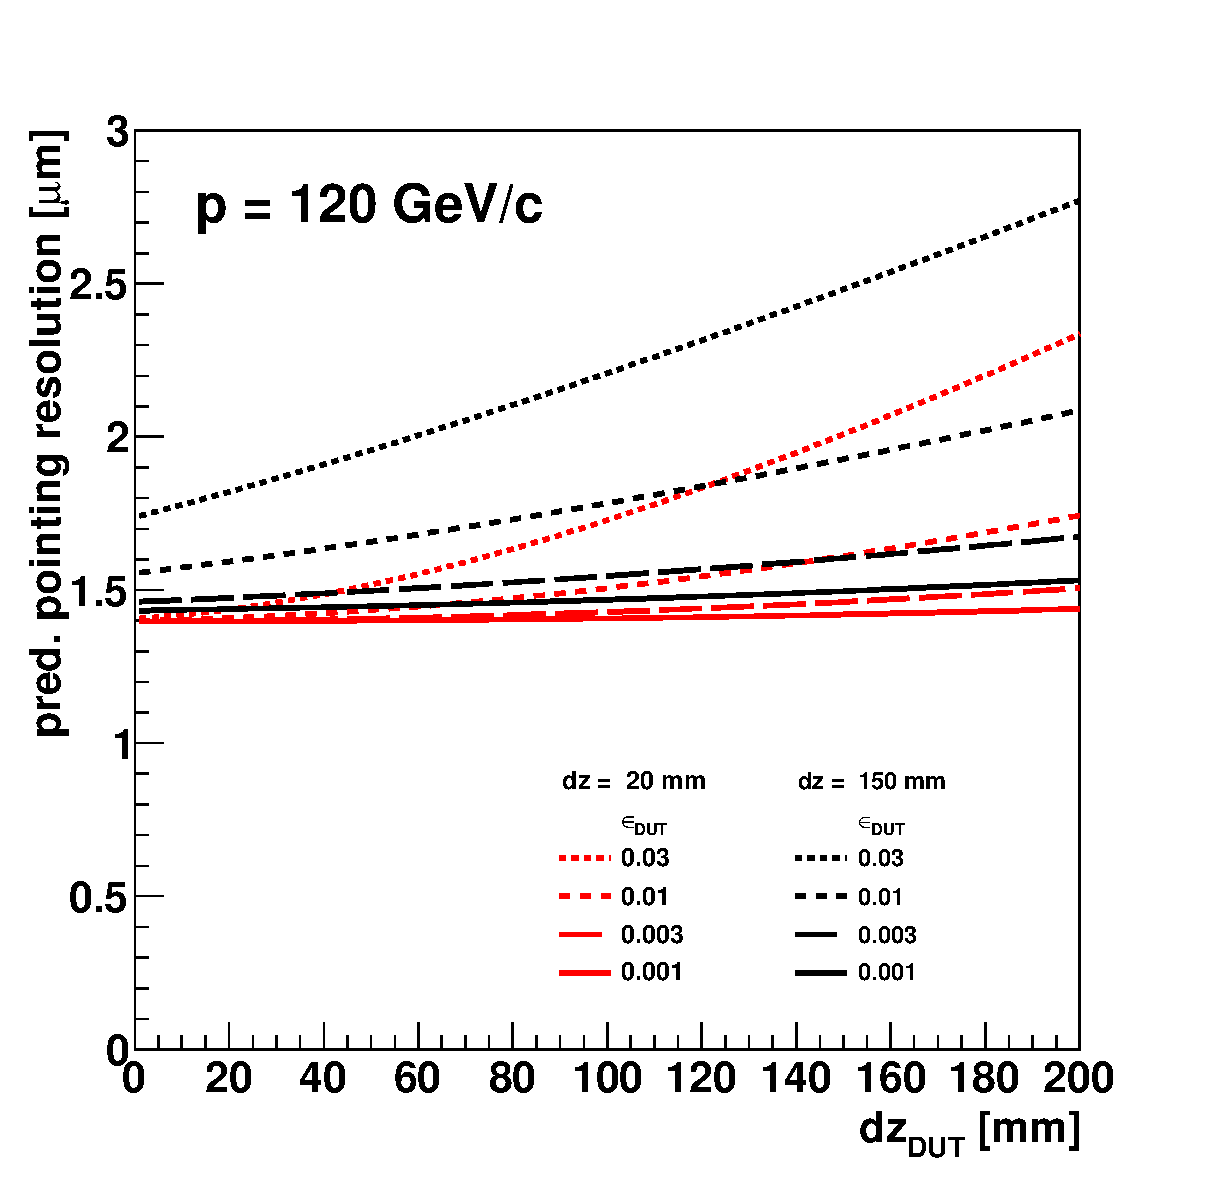
\includegraphics[width=0.49\textwidth]{figures/CalcResoVsDzdut_Cern_2}\\
  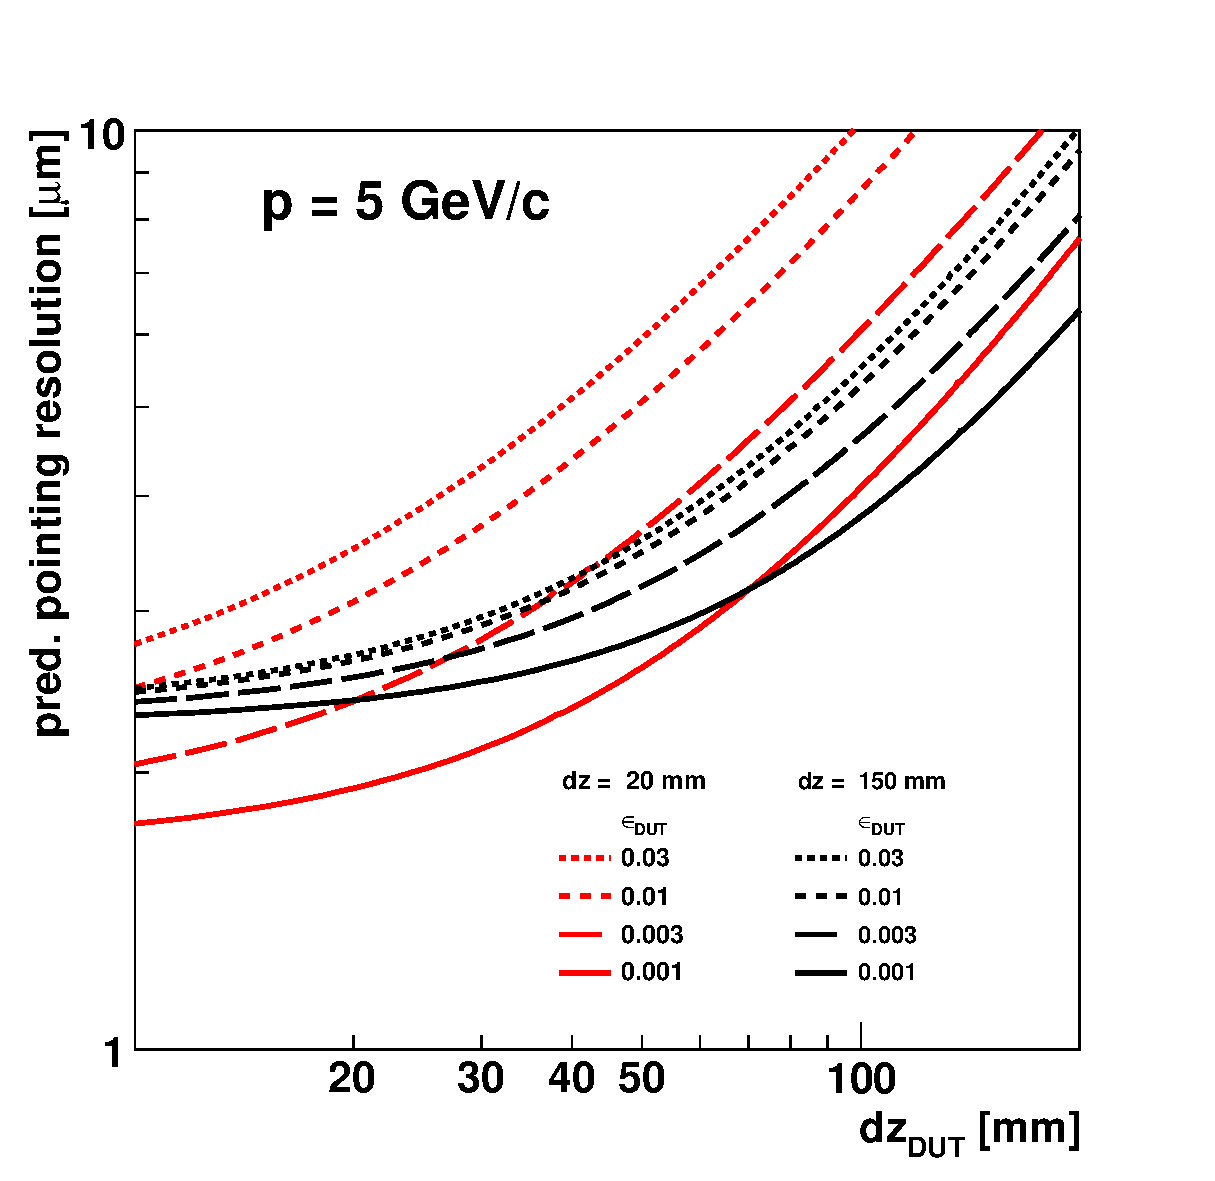
\includegraphics[width=0.49\textwidth]{figures/CalcResoVsDzdut_Desy_loglog_2}
  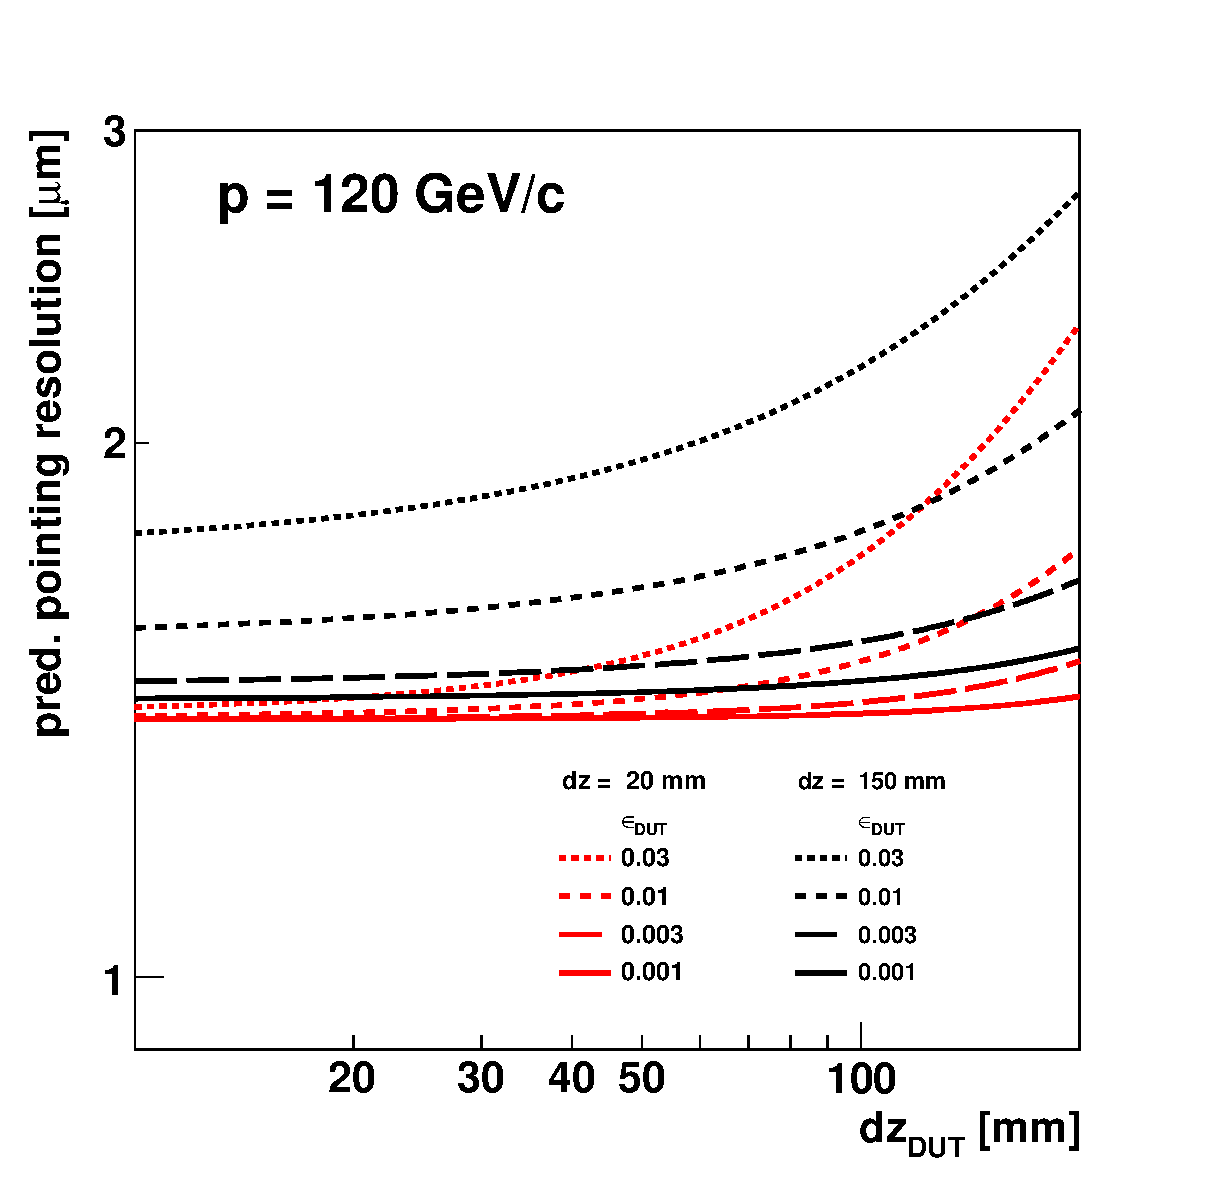
\includegraphics[width=0.49\textwidth]{figures/CalcResoVsDzdut_Cern_loglog_2}
  \caption[Pointing resolution for various DUTs as a function of the distance between DUT and neighbouring planes]{
  The pointing resolution for various DUTs is shown as a function of the equidistant distance between DUT and neighbouring planes.
  Left: at 5\,GeV, Right: at 120\,GeV. }
\label{fig:CalcResos_dzdut}
\end{figure}

A comparison between the measured resolution at the DUT with the calculated pointing resolution $\sigmapGBL$ is only possible, if the measured resolution is corrected by the DUT's resolution

\begin{equation}
 \sigmap = \sqrt{\sigmames^2 - \sigmadut^2}.
 \label{eq:sigmap}
\end{equation}

\noindent
This is shown in figure~\ref{fig:CalcResoP_DUT} (A) as a function of the beam momentum. 
Here, the pointing resolution is analytically calculated for a ``five planes plus DUT'' configuration, where the DUT is a $\Mimosa$ sensor, in order to match the measurements undertaken. 
The solid lines represent GBL calculations, the crosses are the $\sigmap$ corresponding to equation~(\ref{eq:sigmap}). 
The band formed by the solid lines represent the calculated pointing resolution assuming $\sigmai = (3.42 \pm 0.10)\,\upmu\meter$ for the wide and the narrow configuration. 
A nice agreement between the GBL calculations and the pointing resolution derived from the measured resolution is found.
In figure~\ref{fig:CalcResoP_DUT} (B) the achievable pointing resolution as a function of the material budget is plotted from a user's point of view, i.e.~for a ``six planes plus DUT'' configuration. 
Again it can be seen, that a minimal $\dzdut$ allows for the best possible resolution. 
The intersection for equally coloured lines mark the amount of material budget, where a change in the optimal plane spacing $\dz$ happens.
For budgets below (above) the intersection, a narrow (wide) configuration is preferred.
The position of the intersection shifts to smaller material budgets with increasing $\dzdut$. 

\begin{figure}[tbp]
  \centering
  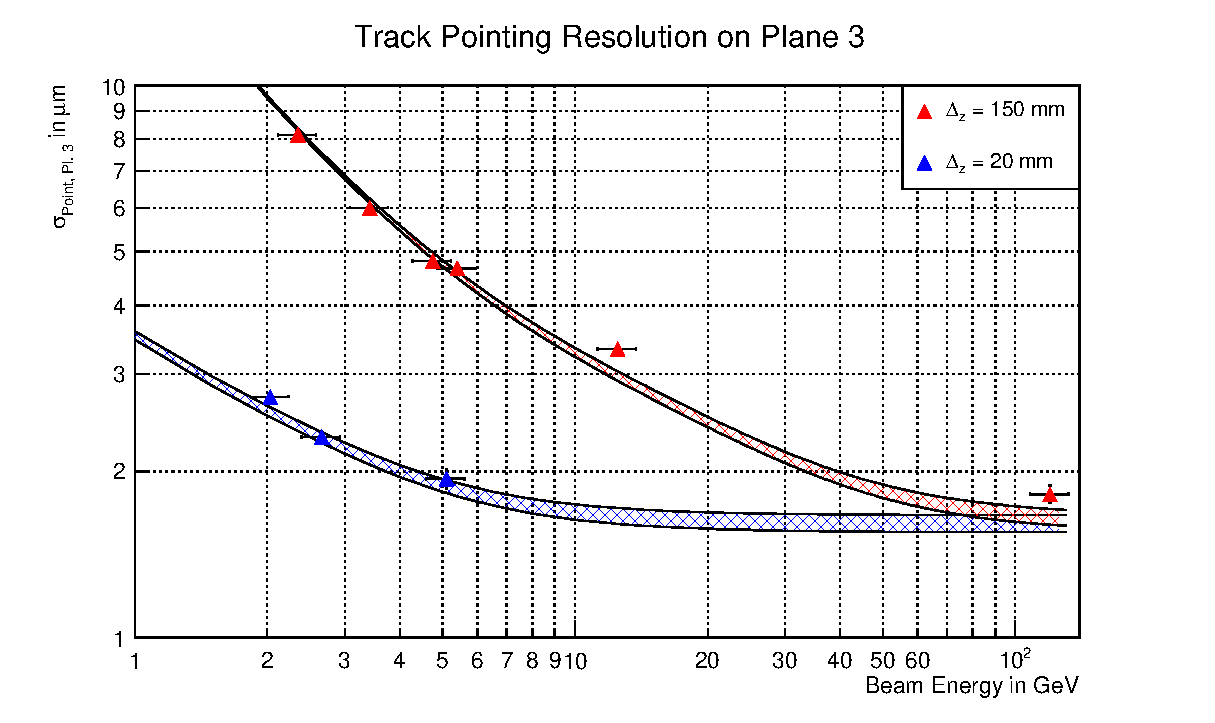
\includegraphics[width=0.49\textwidth]{figures/energy_plot}     \put(-125,175){(A)}
  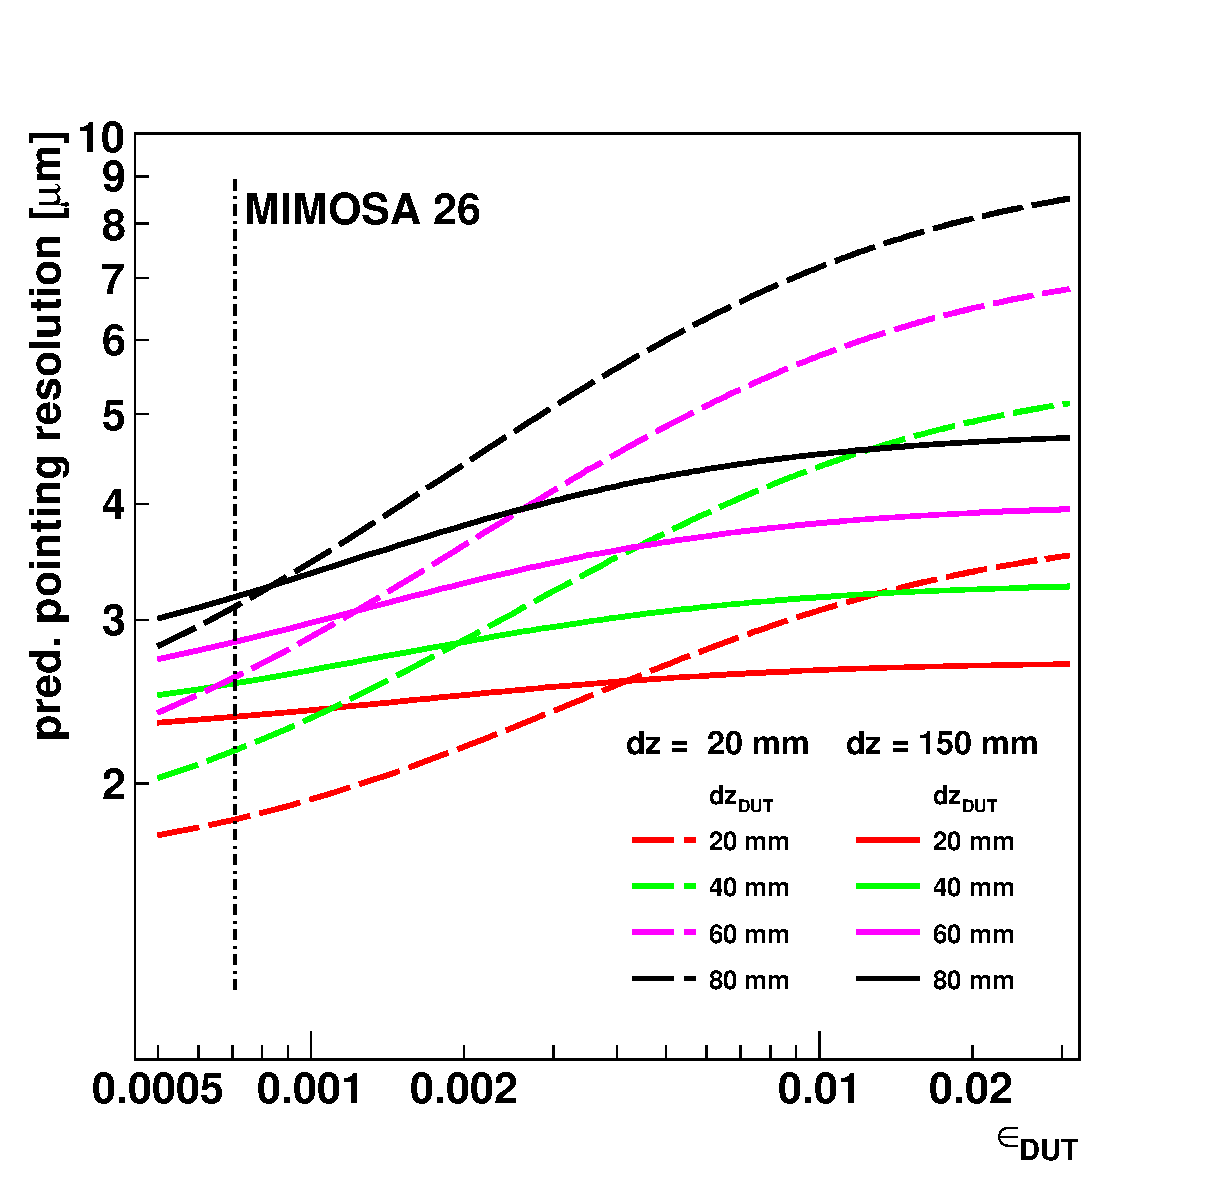
\includegraphics[width=0.49\textwidth]{figures/CalcResoVsEpsdut}\put(-125,175){(B)}
  \caption[Pointing resolution as a function of the beam energy]{
  (A) The pointing resolution for the wide (red) and the narrow (black) set-up is shown as a function of the beam energy for a 5-plane set-up for comparison with data. 
  The theoretical limit of about $1.6\,\upmu\meter$ for plane\,3 is indicated as a dashed line.
  Pointing resolutions derived from the measured resolutions at plane 3 for various energies and plane spacings are shown as crosses.
  (B) The pointing resolution for various geometries is shown as a function of $\epsdut$ for a 6-plane set-up.}
\label{fig:CalcResoP_DUT}
\end{figure}

Take note, that if straight line fitting is used, the inclusion of downstream planes might significantly deteriorate the unbiased residual widths,
 as kinks at the possibly thick DUT (and also the $\Mimosa$ planes themselves) are not allowed for in the fit.
Therefore, using GBL is always recommended. 
If straight line fitting is used nonetheless, a fit using the upstream planes only might result in a better unbiased residual width, compared to a fit that includes the downstream planes.
However, in a narrow ``six planes plus DUT'' set-up using a 5\,GeV beam, the pointing resolution at the DUT using GBL is $1.83\,\upmu\meter$, compared to more than $3.88\,\upmu\meter$ using only the upstream planes.
N.B., that in the ``upstream only'' case, the optimal plane distance is the wide configuration.
A web tool is available with compatible results in comparison with the GBL calculations is available.\,\cite{webtool}


comment hj:\\
apply energy correction (Ref Summer Student 2013) , then re-do reso vs energy plot
